% !TeX program = xelatex
% 第十九章 含参变量的积分
\chapter{含参变量的积分}

为了表示函数，特别是非初等函数，我们曾经系统研究过函数项级数．函数项级数是指
\[
\sum_{n=1}^{\infty}u_{n}(x).
\]
我们已经知道，对每个 $n$，$u_{n}(x)$ 可能是很简单的函数，例如 $a_{n}x^{n}$ 或 $a_{n}\cos nx+b_{n}\sin nx$，但无穷项加起来后，却可以表示极其复杂的函数．本章研究的含参变量积分，与函数项级数十分类似，其区别之处是，级数是对离散量 $n$ 求和，而我们这里是对连续量求积分．当这种积分是有穷区间上的正常积分时，由于已有了多元函数与微积分的理论，研究起来是比较简单的．这是本章 §1 要讲述的内容．当这种积分是无穷区间或有穷区间的广义积分时，情况就同函数项级数更为类似．这时一致收敛的概念成了理论的关键，这是本章 §2 要讲述的内容．应用函数项级数的方法是 §2 的主线，掌握连续变量与离散变量的异同，则是读者学习本节要特别注意的地方．§3 将通过含参变量积分给出两个十分重要的非初等函数——贝塔（Beta）函数和伽玛（Gamma）函数．

\section{含参变量的正常积分}

设函数 $f(x,y)$ 在矩形区域 $[a,b]\times[c,d]$ 上有定义，对 $[a,b]$ 上任一固定的 $x_{0}$，$f(x_{0},y)$ 在 $[c,d]$ 上可积，则
\[
\int_{c}^{d}f(x_{0},y)\dd y
\]
就确定一个数．当 $x$ 在 $[a,b]$ 上变动时，这样的积分就定义了一个函数
\[
I(x)=\int_{c}^{d}f(x,y)\dd y,\quad x\in[a,b],
\]
称此积分为含参变量的积分，参变量为 $x$．

\begin{theorem}[积分号下取极限]\label{thm:19-1}
设 $f(x,y)$ 在矩形区域 $[a,b]\times[c,d]$ 上连续，则
\[
I(x)=\int_{c}^{d}f(x,y)\dd y
\]
在 $[a,b]$ 连续．
\end{theorem}

\begin{proof}
对任意 $x\in[a,b]$，$x+\Delta x\in[a,b]$，有
\[
I(x+\Delta x)-I(x)=\int_{c}^{d}\left[f(x+\Delta x,y)-f(x,y)\right]\dd y.
\]
由于 $f(x,y)$ 在 $[a,b]\times[c,d]$ 连续，因而一致连续，故对任给的 $\varepsilon>0$，存在 $\delta>0$，对任意的 $(x_{1},y_{1})$，$(x_{2},y_{2})\in[a,b]\times[c,d]$，只要 $|x_{1}-x_{2}|<\delta$，$|y_{1}-y_{2}|<\delta$，就有
\[
|f(x_{1},y_{1})-f(x_{2},y_{2})|<\frac{\varepsilon}{d-c}.
\]
因此只要 $|\Delta x|<\delta$，就有
\[
|f(x+\Delta x,y)-f(x,y)|<\frac{\varepsilon}{d-c}
\]
对 $y\in[c,d]$ 都成立，因而
\[
\begin{aligned}
|I(x+\Delta x)-I(x)|&\leqslant\int_{c}^{d}|f(x+\Delta x,y)-f(x,y)|\dd y\\
&<\frac{\varepsilon}{d-c}\int_{c}^{d}\dd y=\varepsilon.
\end{aligned}
\]
这就证明了 $I(x)$ 在 $x$ 点连续．由 $x\in[a,b]$ 的任意性，知 $I(x)$ 在 $[a,b]$ 连续．定理~\ref{thm:19-1} 证完．
\end{proof}

$I(x)$ 在 $[a,b]$ 连续，这等价于说，对任意 $x_{0}\in[a,b]$，有
\[
\lim_{x\to x_{0}}I(x)=I(x_{0}),
\]
即
\[
\lim_{x\to x_{0}}\int_{c}^{d}f(x,y)\dd y=\int_{a}^{b}f(x_{0},y)\dd y=\int_{a}^{b}\lim_{x\to x_{0}}f(x,y)\dd y.
\]
因此，定理 19.1 告诉我们，在定理条件下，求极限和求积分可交换次序．我们也常说求极限可取进积分号内，或说在积分号下取极限．

从几何上看，定理 19.1 是显然的．$z=f(x,y)$ 表示矩形 $[a,b]\times[c,d]$ 上的一块曲面．不妨设 $f(x,y)\geqslant 0$，这时
\[
I(x_{0})=\int_{c}^{d}f(x_{0},y)\dd y
\]
表示平面 $x=x_{0}$ 上，曲面 $z=f(x,y)$ 与平面 $x=x_{0}$ 相交的曲线下方位于 $y=c$ 和 $y=d$ 之间，且 $z\geqslant 0$ 部分的曲边梯形的面积．当曲面是连续时，这个面积 $I(x)$ 显然是 $[a,b]$ 上的连续函数（图~\ref{fig:19-1}）．

\begin{figure}[htbp]
\centering
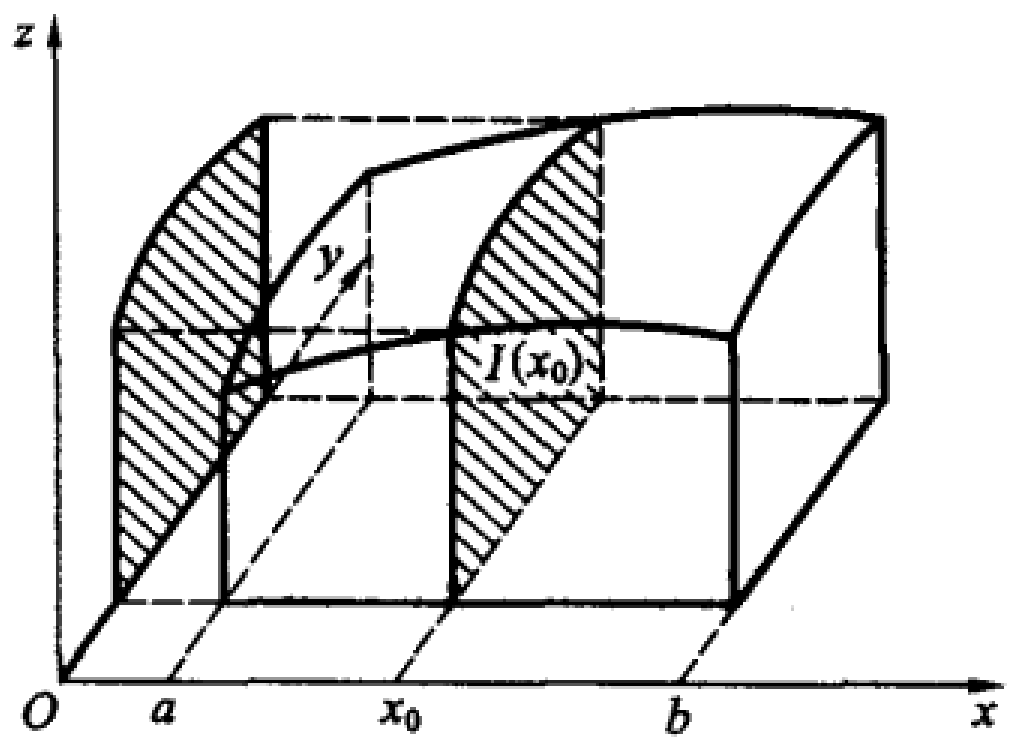
\includegraphics[width=0.45\textwidth]{work/figures/fig19-1}\caption{\relax}\label{fig:19-1}
\end{figure}

\begin{theorem}[积分号下求导数]\label{thm:19-2}
设 $f(x,y)$ 和 $f_{x}(x,y)$ 在 $[a,b]\times[c,d]$ 上连续，则 $I(x)$ 在 $[a,b]$ 有连续的导函数，且
\[
I^{\prime}(x)=\int_{c}^{d}f_{x}(x,y)\dd y.
\]
\end{theorem}

\begin{proof}
对任意 $x\in[a,b]$ 和 $x+\Delta x\in[a,b]$，由拉格朗日中值定理，存在 $\theta\in(0,1)$，使得
\[
\begin{aligned}
\frac{I(x+\Delta x)-I(x)}{\Delta x}&=\int_{c}^{d}\frac{f(x+\Delta x,y)-f(x,y)}{\Delta x}\dd y\\
&=\int_{c}^{d}f_{x}(x+\theta\Delta x,y)\dd y.
\end{aligned}
\]
由函数 $f_{x}(x,y)$ 在 $[a,b]\times[c,d]$ 连续，从而一致连续，即对任给的 $\varepsilon>0$，存在 $\delta>0$，只要 $|\Delta x|<\delta$，有
\[
|f_{x}(x+\theta\Delta x,y)-f_{x}(x,y)|<\frac{\varepsilon}{d-c}
\]
对 $y\in[c,d]$ 同时成立，因此
\[
\begin{aligned}
&\left|\frac{I(x+\Delta x)-I(x)}{\Delta x}-\int_{c}^{d}f_{x}(x,y)\dd y\right|\\
={}&\left|\int_{c}^{d}\left[f_{x}(x+\theta\Delta x,y)-f_{x}(x,y)\right]\dd y\right|\\
\leqslant{}&\int_{c}^{d}\left|f_{x}(x+\theta\Delta x,y)-f_{x}(x,y)\right|\dd y\\
<{}&\frac{\varepsilon}{d-c}\int_{c}^{d}\dd y=\varepsilon.
\end{aligned}
\]
故 $I(x)$ 在 $x$ 可导，且
\[
I^{\prime}(x)=\int_{c}^{d}f_{x}(x,y)\dd y.
\]
由 $x\in[a,b]$ 的任意性及定理 19.1 知，$I(x)$ 在 $[a,b]$ 有连续的导函数，且上式成立．定理~\ref{thm:19-2} 证完．
\end{proof}

定理 19.2 的结论又可写为
\[
\frac{\dd}{\dd x}\int_{c}^{d}f(x,y)\dd y=\int_{c}^{d}f_{x}(x,y)\dd y=\int_{c}^{d}\frac{\partial}{\partial x}f(x,y)\dd y.
\]
这说明，在定理的条件下，求导和求积分可交换次序．我们也常说可在积分号下求导数．

\begin{example}\label{ex:19-1-1}
求 $I(\theta)=\int_{0}^{\pi}\ln(1+\theta\cos x)\dd x$，其中 $|\theta|<1$．
\end{example}

\begin{proof}[解]
对任意 $|\theta|<1$，存在 $b$ 使得 $|\theta|<b<1$．于是
\[
f(x,\theta)=\ln(1+\theta\cos x),\quad f_{\theta}(x,\theta)=\frac{\cos x}{1+\theta\cos x}
\]
都在 $[0,\pi]\times[-b,b]$ 连续，由定理 19.2 得
\[
I^{\prime}(\theta)=\int_{0}^{\pi}\frac{\cos x}{1+\theta\cos x}\dd x.
\]
当 $\theta\neq 0$ 时
\[
\begin{aligned}
I^{\prime}(\theta)&=\frac{1}{\theta}\int_{0}^{\pi}\left(1-\frac{1}{1+\theta\cos x}\right)\dd x\\
&=\frac{\pi}{\theta}-\frac{1}{\theta}\int_{0}^{\pi}\frac{\dd x}{1+\theta\cos x}.
\end{aligned}
\]
令 $\tan\dfrac{x}{2}=t$，则
\[
\begin{aligned}
\int_{0}^{\pi}\frac{\dd x}{1+\theta\cos x}&=\int_{0}^{+\infty}\frac{1}{1+\theta\dfrac{1-t^{2}}{1+t^{2}}}\cdot\frac{2}{1+t^{2}}\dd t\\
&=\int_{0}^{+\infty}\frac{2\dd t}{(1+\theta)+(1-\theta)t^{2}}=\left.\frac{2}{\sqrt{1-\theta^{2}}}\arctan\sqrt{\frac{1-\theta}{1+\theta}}\,t\right|_{0}^{+\infty}\\
&=\frac{\pi}{\sqrt{1-\theta^{2}}}.
\end{aligned}
\]
因此
\[
I^{\prime}(\theta)=\frac{\pi}{\theta}-\frac{\pi}{\theta\sqrt{1-\theta^{2}}}=\frac{-\theta\pi}{\sqrt{1-\theta^{2}}\left(1+\sqrt{1-\theta^{2}}\right)},
\]
积分得
\[
\begin{aligned}
I(\theta)&=\int\frac{-\theta\pi\dd\theta}{\sqrt{1-\theta^{2}}\left(1+\sqrt{1-\theta^{2}}\right)}\\
&=\pi\int\frac{\dd\sqrt{1-\theta^{2}}}{1+\sqrt{1-\theta^{2}}}\\
&=\pi\ln\left(1+\sqrt{1-\theta^{2}}\right)+C,\ \theta\in[-b,b],\ \theta\neq 0.
\end{aligned}
\]
又由 $I(0)=0$ 及 $I(\theta)$ 的连续性得 $C=-\pi\ln 2$，因此
\[
I(\theta)=\pi\ln\frac{1+\sqrt{1-\theta^{2}}}{2},\quad|\theta|<1.
\]
\end{proof}

我们发现，用含参变量积分给出的 $I(\theta)$，原来是一个初等函数．这一点，用一元函数的积分知识是不容易看出来的．我们用了含参变量积分的理论（积分号下求导数），才把它计算出来．

\begin{example}\label{ex:19-1-2}
计算定积分
\[
I=\int_{0}^{1}\frac{\ln(1+x)}{1+x^{2}}\dd x.
\]
\end{example}

\begin{proof}[解]
这个积分并不带参变量，但被积函数的原函数不能用初等函数表示．为此，引入参变量，考虑含参变量积分
\[
I(\alpha)=\int_{0}^{1}\frac{\ln(1+\alpha x)}{1+x^{2}}\dd x,\quad\alpha\in[0,1].
\]
我们将通过积分号下求导数，再求出 $I=I(1)$．记
\[
f(x,\alpha)=\frac{\ln(1+\alpha x)}{1+x^{2}},
\]
则
\[
f_{\alpha}(x,\alpha)=\frac{x}{(1+x^{2})(1+\alpha x)}=\frac{1}{1+\alpha^{2}}\left(\frac{\alpha+x}{1+x^{2}}-\frac{\alpha}{1+\alpha x}\right)
\]
它们都在 $[0,1]\times[0,1]$ 上连续，根据定理 19.2，有
\[
\begin{aligned}
I^{\prime}(\alpha)&=\int_{0}^{1}f_{\alpha}(x,\alpha)\dd x\\
&=\int_{0}^{1}\frac{1}{1+\alpha^{2}}\left(\frac{\alpha+x}{1+x^{2}}-\frac{\alpha}{1+\alpha x}\right)\dd x\\
&=\frac{1}{1+\alpha^{2}}\left[\alpha\arctan x+\frac{1}{2}\ln(1+x^{2})-\ln(1+\alpha x)\right]\bigg|_{0}^{1}\\
&=\frac{1}{1+\alpha^{2}}\left[\frac{\pi}{4}\alpha+\frac{1}{2}\ln 2-\ln(1+\alpha)\right].
\end{aligned}
\]
注意到 $I(0)=0$，故
\[
\begin{aligned}
I(1)&=I(1)-I(0)=\int_{0}^{1}I^{\prime}(\alpha)\dd\alpha\\
&=\int_{0}^{1}\frac{1}{1+\alpha^{2}}\left[\frac{\pi}{4}\alpha+\frac{1}{2}\ln 2-\ln(1+\alpha)\right]\dd\alpha\\
&=\left[\frac{\pi}{8}\ln(1+\alpha^{2})+\frac{1}{2}\ln 2\arctan\alpha\right]\bigg|_{0}^{1}-\int_{0}^{1}\frac{\ln(1+\alpha)}{1+\alpha^{2}}\dd\alpha\\
&=\frac{\pi}{8}\ln 2+\frac{\pi}{8}\ln 2-I(1)=\frac{\pi}{4}\ln 2-I(1),
\end{aligned}
\]
从而
\[
I=I(1)=\frac{\pi}{8}\ln 2.
\]
\end{proof}

下面我们进一步考虑含参变量积分的积分限也依赖于参数 $x$ 的情形．为此先考虑函数
\[
I(x,u)=\int_{c}^{u}f(x,y)\dd y
\]
的性质．

\begin{theorem}\label{thm:19-3}
设函数 $f(x,y)$ 在矩形区域 $[a,b]\times[c,d]$ 上连续，
\[
I(x,u)=\int_{c}^{u}f(x,y)\dd y,
\]
则（1）$I(x,u)$ 在 $[a,b]\times[c,d]$ 上连续；

（2）若 $f_{x}(x,y)$ 在 $[a,b]\times[c,d]$ 上连续，则 $I(x,u)$ 在 $[a,b]\times[c,d]$ 对各变元有连续偏导数．
\end{theorem}

\begin{proof}
（1）对任意 $(x_{0},u_{0})$，$(x,u)\in[a,b]\times[c,d]$，则
\[
\begin{aligned}
&|I(x,u)-I(x_{0},u_{0})|=\left|\int_{c}^{u}f(x,y)\dd y-\int_{c}^{u_{0}}f(x_{0},y)\dd y\right|\\
={}&\left|\int_{c}^{u_{0}}\left[f(x,y)-f(x_{0},y)\right]\dd y+\int_{u_{0}}^{u}f(x,y)\dd y\right|.
\end{aligned}
\]
由 $f(x,y)$ 在 $[a,b]\times[c,d]$ 上连续，因而有界且一致连续，知存在 $M>0$，使
\[
|f(x,y)|\leqslant M,\quad(x,y)\in[a,b]\times[c,d],
\]
且对任给的 $\varepsilon>0$，存在 $\delta_{1}>0$，对任意的 $(x_{1},y_{1})$，$(x_{2},y_{2})\in[a,b]\times[c,d]$，只要 $|x_{1}-x_{2}|<\delta_{1}$ 和 $|y_{1}-y_{2}|<\delta_{1}$，就有
\[
|f(x_{1},y_{1})-f(x_{2},y_{2})|<\frac{\varepsilon}{2(d-c)}.
\]
取 $\delta=\min\left(\delta_{1},\dfrac{\varepsilon}{2M}\right)$，则当 $|x-x_{0}|<\delta$，$|u-u_{0}|<\delta$ 时，有
\[
\begin{aligned}
&|I(x,u)-I(x_{0},u_{0})|\\
\leqslant{}&\int_{c}^{u_{0}}|f(x,y)-f(x_{0},y)|\dd y+M\left|\int_{u_{0}}^{u}\dd y\right|\\
<{}&\frac{\varepsilon}{2(d-c)}(u_{0}-c)+M\frac{\varepsilon}{2M}\leqslant\frac{\varepsilon}{2}+\frac{\varepsilon}{2}=\varepsilon.
\end{aligned}
\]
即 $I(x,u)$ 在 $(x_{0},u_{0})$ 点连续．由 $(x_{0},u_{0})\in[a,b]\times[c,d]$ 的任意性，便证得 $I(x,u)$ 在 $[a,b]\times[c,d]$ 上连续．

（2）由微积分基本定理，$I$ 对 $u$ 有连续的偏导数
\[
\frac{\partial I}{\partial u}=f(x,u).
\]
又由定理 19.2，$I$ 对 $x$ 也有连续的偏导数
\[
\frac{\partial I}{\partial x}=\int_{c}^{u}f_{x}(x,y)\dd y.
\]
这就是所要证明的，定理~\ref{thm:19-3} 证完．
\end{proof}

利用定理 19.3 及复合函数的连续性与求导数的链式法则，立即可得下面两个定理．

\begin{theorem}\label{thm:19-4}
设函数 $f(x,y)$ 在 $[a,b]\times[c,d]$ 上连续，$c(x)$，$d(x)$ 都在 $[a,b]$ 上连续，并且当 $x\in[a,b]$ 时，有
\[
c\leqslant c(x),\ d(x)\leqslant d,
\]
则
\[
F(x)=\int_{c(x)}^{d(x)}f(x,y)\dd y
\]
在 $[a,b]$ 连续．
\end{theorem}

\begin{proof}
令 $u=d(x)$，$v=c(x)$，$I(x,u)=\int_{c}^{u}f(x,y)\dd y$．根据定理 19.3，
\[
\int_{v}^{u}f(x,y)\dd y=\int_{c}^{u}f(x,y)\dd y-\int_{c}^{v}f(x,y)\dd y=I(x,u)-I(x,v)
\]
在 $[a,b]\times[c,d]\times[c,d]$ 上连续．由复合函数的连续性知
\[
F(x)=I(x,d(x))-I(x,c(x))
\]
在 $[a,b]$ 连续．定理~\ref{thm:19-4} 证完．
\end{proof}

\begin{theorem}\label{thm:19-5}
设函数 $f(x,y)$，$f_{x}(x,y)$ 都在 $[a,b]\times[c,d]$ 上连续，又 $c^{\prime}(x)$ 和 $d^{\prime}(x)$ 在 $[a,b]$ 存在，且当 $x\in[a,b]$ 时，有
\[
c\leqslant c(x),\ d(x)\leqslant d,
\]
则
\[
F(x)=\int_{c(x)}^{d(x)}f(x,y)\dd y
\]
在 $[a,b]$ 可导，且
\[
F^{\prime}(x)=\int_{c(x)}^{d(x)}f_{x}(x,y)\dd y+f(x,d(x))d^{\prime}(x)-f(x,c(x))c^{\prime}(x).
\]
\end{theorem}

\begin{proof}
令
\[
I(x,u)=\int_{c}^{u}f(x,y)\dd y,\quad H(x,u,v)=\int_{v}^{u}f(x,y)\dd y.
\]
则 $H(x,u,v)=I(x,u)-I(x,v)$．由定理 19.3，$H$ 对各变元有连续的偏导数．又 $c(x)$，$d(x)$ 在 $[a,b]$ 可导，且当 $x\in[a,b]$ 时，
\[
c\leqslant c(x),\ d(x)\leqslant d,
\]
故由复合函数求导数的链式法则，$F(x)=H(x,c(x),d(x))$ 在 $[a,b]$ 可导，且
\[
\begin{aligned}
F^{\prime}(x)&=\frac{\partial H}{\partial x}+\frac{\partial H}{\partial u}d^{\prime}(x)+\frac{\partial H}{\partial v}c^{\prime}(x)\\
&=\int_{c(x)}^{d(x)}f_{x}(x,y)\dd y+f(x,d(x))d^{\prime}(x)-f(x,c(x))c^{\prime}(x).
\end{aligned}
\]
定理~\ref{thm:19-5} 证完．
\end{proof}

其实，定理 19.4、19.5 也可以不用定理 19.3 而直接证明，作为一个练习，请读者把它们写出来．

\begin{example}\label{ex:19-1-3}
设 $F(x)=\int_{x}^{x^{2}}\dfrac{\sin xy}{y}\dd y$，求 $F^{\prime}(x)$．
\end{example}

\begin{proof}[解]
这个积分是积不出来的，但用定理 19.5 有
\[
\begin{aligned}
F^{\prime}(x)&=\int_{x}^{x^{2}}\cos xy\dd y+2x\left(\frac{\sin x^{3}}{x^{2}}\right)-\frac{\sin x^{2}}{x}\\
&=\frac{1}{x}\sin xy\bigg|_{x}^{x^{2}}+\frac{2\sin x^{3}}{x}-\frac{\sin x^{2}}{x}\\
&=\frac{3\sin x^{3}-2\sin x^{2}}{x}.
\end{aligned}
\]
\end{proof}

\begin{example}\label{ex:19-1-4}
设 $f(x)$ 在 $x=0$ 的某邻域内连续，则微分方程
\[
\begin{cases}
y^{(n)}(x)=f(x),\\
y(0)=0,\quad y^{\prime}(0)=0,\quad\cdots,\quad y^{(n-1)}(0)=0
\end{cases}
\]
的解在 $x=0$ 附近可表示成
\[
y(x)=\frac{1}{(n-1)!}\int_{0}^{x}(x-t)^{n-1}f(t)\dd t,
\]
其中 $n$ 是任意正整数．
\end{example}

\begin{proof}
利用定理 19.5，则
\[
\begin{aligned}
y^{\prime}(x)&=\frac{1}{(n-1)!}\int_{0}^{x}(n-1)(x-t)^{n-2}f(t)\dd t\\
&\quad+\frac{1}{(n-1)!}(x-x)^{n-1}f(x)\\
&=\frac{1}{(n-2)!}\int_{0}^{x}(x-t)^{n-2}f(t)\dd t.
\end{aligned}
\]
一般地有
\[
y^{(k)}(x)=\frac{1}{(n-k-1)!}\int_{0}^{x}(x-t)^{n-k-1}f(t)\dd t,
\]
从而
\[
y^{(n-1)}(x)=\int_{0}^{x}f(t)\dd t,
\]
\[
y^{(n)}(x)=f(x).
\]
显然
\[
y(0)=y^{\prime}(0)=\cdots=y^{(k)}(0)=\cdots=y^{(n-1)}(0)=0.
\]
\end{proof}

最后我们来讨论含参变量积分 $I(x)=\int_{c}^{d}f(x,y)\dd y$ 的积分问题．如果 $I(x)$ 在 $[a,b]$ 可积，通常把它在 $[a,b]$ 的积分写为
\[
\int_{a}^{b}I(x)\dd x=\int_{a}^{b}\left[\int_{c}^{d}f(x,y)\dd y\right]\dd x=\int_{a}^{b}\dd x\int_{c}^{d}f(x,y)\dd y,
\]
称之为先对 $y$ 后对 $x$ 的累次积分．

\begin{theorem}[积分交换次序]\label{thm:19-6}
设 $f(x,y)$ 在 $[a,b]\times[c,d]$ 上连续，
\[
I(x)=\int_{c}^{d}f(x,y)\dd y,
\]
则
\[
\int_{a}^{b}I(x)\dd x=\int_{c}^{d}\dd y\int_{a}^{b}f(x,y)\dd x,
\]
即
\[
\int_{a}^{b}\dd x\int_{c}^{d}f(x,y)\dd y=\int_{c}^{d}\dd y\int_{a}^{b}f(x,y)\dd x.
\]
\end{theorem}

\begin{proof}
由定理 19.1，$I(x)$ 在 $[a,b]$ 连续，因而是可积的，令
\[
I_{1}(u)=\int_{a}^{u}\dd x\int_{c}^{d}f(x,y)\dd y,\ u\in[a,b],
\]
\[
I_{2}(u)=\int_{c}^{d}\dd y\int_{a}^{u}f(x,y)\dd x,\ u\in[a,b].
\]
由定理 19.1 知，$\displaystyle\int_{c}^{d}f(x,y)\dd y$ 在 $[a,b]$ 连续，因此 $I_{1}(u)$ 在 $[a,b]$ 可导，且
\[
I_{1}^{\prime}(u)=\int_{c}^{d}f(u,y)\dd y,
\]
又由定理 19.3 知，$\displaystyle\int_{a}^{u}f(x,y)\dd x$ 关于变量 $y$，$u$ 二元连续，其关于 $u$ 的偏导数 $f(u,y)$ 也是连续的，从而由定理 19.2 知，$I_{2}(u)$ 在 $[a,b]$ 可导，且
\[
I_{2}^{\prime}(u)=\int_{c}^{d}\frac{\partial}{\partial u}\int_{a}^{u}f(x,y)\dd x\dd y=\int_{c}^{d}f(u,y)\dd y.
\]
这就证明了
\[
I_{1}^{\prime}(u)=I_{2}^{\prime}(u),\ u\in[a,b].
\]
因此
\[
I_{1}(u)=I_{2}(u)+c,\quad u\in[a,b].
\]
令 $u=a$，由 $I_{1}(a)=I_{2}(a)=0$ 推得 $c=0$．故
\[
I_{1}(u)=I_{2}(u),\quad u\in[a,b].
\]
令 $u=b$，即得
\[
\int_{a}^{b}\dd x\int_{c}^{d}f(x,y)\dd y=\int_{c}^{d}\dd y\int_{a}^{b}f(x,y)\dd x.
\]
定理~\ref{thm:19-6} 证完．
\end{proof}

定理 19.6 说明：在被积函数二元连续的条件下，两个累次积分可以交换次序．

\begin{example}\label{ex:19-1-5}
用积分交换次序求解例 1，即求
\[
I(\theta)=\int_{0}^{\pi}\ln(1+\theta\cos x)\dd x,
\]
其中 $|\theta|<1$．
\end{example}

\begin{proof}[解]
显然 $I(\theta)=\displaystyle\int_{0}^{\pi}\dd x\int_{0}^{\theta}\frac{\cos x}{1+y\cos x}\dd y$．令
\[
f(x,y)=\frac{\cos x}{1+y\cos x},
\]
因为 $f(x,y)$ 在 $[0,\pi]\times[0,\theta]$ 上连续，所以积分可交换次序，
\[
I(\theta)=\int_{0}^{\theta}\dd y\int_{0}^{\pi}\frac{\cos x}{1+y\cos x}\dd x.
\]
用变量代换，在例 1 中已求出
\[
\int_{0}^{\pi}\frac{\cos x}{1+y\cos x}\dd x=\frac{-y\pi}{\sqrt{1-y^{2}}\left(1+\sqrt{1-y^{2}}\right)},
\]
因此
\[
\begin{aligned}
I(\theta)&=\int_{0}^{\theta}\frac{-y\pi}{\sqrt{1-y^{2}}\left(1+\sqrt{1-y^{2}}\right)}\dd y\\
&=\pi\int_{0}^{\theta}\frac{\dd\sqrt{1-y^{2}}}{1+\sqrt{1-y^{2}}}=\pi\ln\left(1+\sqrt{1-y^{2}}\right)\bigg|_{0}^{\theta}\\
&=\pi\ln\frac{1+\sqrt{1-\theta^{2}}}{2}.
\end{aligned}
\]
\end{proof}

\begin{xiti}
\item 求下列极限：
\begin{ziti}
\item $\lim\limits_{a\to 0}\displaystyle\int_{-1}^{1}\sqrt{x^{2}+a^{2}}\dd x$；
\item $\lim\limits_{a\to 0}\displaystyle\int_{0}^{2}x^{2}\cos ax\dd x$；
\item $\lim\limits_{a\to 0}\displaystyle\int_{a}^{1+a}\frac{\dd x}{1+x^{2}+a^{2}}$．
\end{ziti}
\item 求 $F^{\prime}(x)$，其中：
\begin{ziti}
\item $F(x)=\displaystyle\int_{x}^{x^{2}}\mathrm{e}^{-xy^{2}}\dd y$；
\item $F(x)=\displaystyle\int_{\sin x}^{\cos x}\mathrm{e}^{x\sqrt{1-y^{2}}}\dd y$；
\item $F(x)=\displaystyle\int_{a+x}^{b+x}\frac{\sin(xy)}{y}\dd y$；
\item $F(x)=\displaystyle\int_{0}^{x}\left[\int_{t^{2}}^{x}f(t,s)\dd s\right]\dd t$．
\end{ziti}
\item 设 $f(x)$ 为连续函数，$h>0$，
\[
F(x)=\int_{0}^{h}\left[\int_{0}^{h}f(x+\xi+\eta)\dd\eta\right]\dd\xi,
\]
求 $F^{\prime\prime}(x)$．
\item 研究函数
\[
F(y)=\int_{0}^{1}\frac{yf(x)}{x^{2}+y^{2}}\dd x
\]
的连续性，其中 $f(x)$ 是 $[0,1]$ 上连续且为正的函数．
\item 应用积分号下求导法求下列积分：
\begin{ziti}
\item $\displaystyle\int_{0}^{\frac{\pi}{2}}\ln(a^{2}-\sin^{2}x)\dd x$ $(a>1)$；
\item $\displaystyle\int_{0}^{\pi}\ln(1-2a\cos x+a^{2})\dd x$ $(|a|<1)$；
\item $\displaystyle\int_{0}^{\frac{\pi}{2}}\ln(a^{2}\sin^{2}x+b^{2}\cos^{2}x)\dd x$ $(a,b\neq 0)$；
\item $\displaystyle\int_{0}^{\frac{\pi}{2}}\frac{\arctan(a\tan x)}{\tan x}\dd x$ $(|a|<1)$．
\end{ziti}
\item 应用积分交换次序求下列积分：
\begin{ziti}
\item $\displaystyle\int_{0}^{1}\frac{x^{b}-x^{a}}{\ln x}\dd x$ $(a>0,\ b>0)$；
\item $\displaystyle\int_{0}^{1}\sin\left(\ln\frac{1}{x}\right)\frac{x^{b}-x^{a}}{\ln x}\dd x$ $(a>0,\ b>0)$．
\end{ziti}
\item 设 $f$ 为可微函数，试求下列函数的二阶导数：
\begin{ziti}
\item $F(x)=\displaystyle\int_{0}^{x}(x+y)f(y)\dd y$；
\item $F(x)=\displaystyle\int_{a}^{b}f(y)\left|x-y\right|\dd y$ $(a<b)$．
\end{ziti}
\item 证明：$\displaystyle\int_{0}^{1}\dd x\int_{0}^{1}\frac{x^{2}-y^{2}}{(x^{2}+y^{2})^{2}}\dd y\neq\int_{0}^{1}\dd y\int_{0}^{1}\frac{x^{2}-y^{2}}{(x^{2}+y^{2})^{2}}\dd x$．
\item 设 $F(y)=\displaystyle\int_{0}^{1}\ln\sqrt{x^{2}+y^{2}}\dd x$，问是否成立
\[
F^{\prime}(0)=\int_{0}^{1}\frac{\partial}{\partial y}\ln\sqrt{x^{2}+y^{2}}\bigg|_{y=0}\dd x.
\]
\item 设
\[
F(x)=\int_{0}^{2\pi}\mathrm{e}^{x\cos\theta}\cos(x\sin\theta)\dd\theta,
\]
求证 $F(x)\equiv 2\pi$．
\item 设 $f(x)$ 为两次可微函数，$\varphi(x)$ 为可微函数，证明函数
\[
u(x,t)=\frac{1}{2}\left[f(x-at)+f(x+at)\right]+\frac{1}{2a}\int_{x-at}^{x+at}\varphi(z)\dd z
\]
满足弦振动方程
\[
\frac{\partial^{2}u}{\partial t^{2}}=a^{2}\frac{\partial^{2}u}{\partial x^{2}}
\]
及初始条件
\[
u(x,0)=f(x),\quad u_{t}(x,0)=\varphi(x).
\]
\end{xiti}

\section{含参变量的广义积分}

\subsection{一致收敛}

广义积分有两种，一种是无穷限积分，即积分区间为无穷的情形，另一种为瑕积分，即积分区间虽然是有穷的，但被积函数在积分区间内无界．当含参变量的积分是广义积分时，就称为含参变量的广义积分．它自然包括两种．

设 $f(x,y)$ 定义在 $[a,b]\times[c,+\infty)$，则
\[
I(x)=\int_{c}^{+\infty}f(x,y)\dd y
\]
为无穷限的含参变量积分，其中 $x$ 是参变量，$y$ 是积分变量．如果 $f(x,y)$ 定义在 $[a,b]\times[c,d]$，且对任意 $x\in[a,b]$ 以及 $\eta>0$ 充分小，$f(x,y)$ 对 $y$ 在 $[c,d-\eta]$ 可积，但在 $[d-\eta,d)$ 无界，则
\[
J(x)=\int_{c}^{d}f(x,y)\dd y
\]
是含参变量的瑕积分．根据广义积分的定义
\[
\int_{c}^{+\infty}f(x,y)\dd y=\lim_{A\to+\infty}\int_{c}^{A}f(x,y)\dd y,
\]
\[
\int_{c}^{d}f(x,y)\dd y=\lim_{\eta\to 0^{+}}\int_{c}^{d-\eta}f(x,y)\dd y,
\]
它们都是含参变量正常积分的极限，这与函数项级数
\[
\sum_{k=1}^{\infty}u_{k}(x),\ x\in[a,b]
\]
十分类似，它是有限和（部分和）的极限
\[
\sum_{k=1}^{\infty}u_{k}(x)=\lim_{n\to\infty}\sum_{k=1}^{n}u_{k}(x).
\]
唯一的差别是，在级数的情形，极限是对离散量 $n\to\infty$ 取的，而在含参变量广义积分的情形，极限是对连续量 $A\to+\infty$ 或 $\eta\to 0^{+}$ 取的．回忆函数项级数理论，我们研究过它的两个基本问题：（1）收敛区域；（2）和函数在收敛区域的分析性质（连续性、可微性、可积性等）．对含参变量的广义积分，同样地有两个问题，但收敛区域的问题，实际上已在第十一章中讲述过．因此本章主要讨论由广义积分表示的函数的分析性质问题．

回忆函数项级数的情形，在和函数分析性质的研究中，一致收敛的概念起了关键的作用．通过一致收敛，把无穷和的性质化为有限和的研究．在含参变量广义积分的讨论中，我们也引入一致收敛的概念，它把广义积分的问题化归为含参变量的正常积分，而后者在本章 §1 中已讨论过．本章主要讨论无穷限的情形，但所有的结果都可平行地推广到瑕积分的情形．

\begin{definition}\label{def:19-1}
设 $f(x,y)$ 定义在 $[a,b]\times[c,+\infty)$，且对任意 $x\in[a,b]$，无穷积分
\[
I(x)=\int_{c}^{+\infty}f(x,y)\dd y
\]
收敛．若对任意的 $\varepsilon>0$，存在 $A_{0}>c$，当 $A>A_{0}$ 时，有
\[
\left|\int_{c}^{A}f(x,y)\dd y-I(x)\right|<\varepsilon
\]
或
\[
\left|\int_{A}^{+\infty}f(x,y)\dd y\right|<\varepsilon
\]
对 $x\in[a,b]$ 都成立，则称含参变量的广义积分 $\displaystyle\int_{c}^{+\infty}f(x,y)\dd y$ 在 $[a,b]$ 一致收敛．
\end{definition}

显然，定义中的区间 $[a,b]$ 可代之以开区间、半开区间、无穷区间等等．

\begin{example}\label{ex:19-2-1}
证明含参变量广义积分 $\displaystyle\int_{0}^{+\infty}x\mathrm{e}^{-xy}\dd y$

（1）在 $[a,+\infty)$ 一致收敛，其中 $a>0$；

（2）在 $(0,+\infty)$ 不一致收敛．
\end{example}

\begin{proof}
（1）因为
\[
\int_{A}^{+\infty}x\mathrm{e}^{-xy}\dd y=-\left.\mathrm{e}^{-xy}\right|_{A}^{+\infty}=\mathrm{e}^{-xA}\leqslant\mathrm{e}^{-aA},\ x\geqslant a,
\]
而 $\lim\limits_{A\to+\infty}\mathrm{e}^{-aA}=0$，所以对任给的 $\varepsilon>0$，存在 $A_{0}>0$，当 $A>A_{0}$ 时有 $\mathrm{e}^{-aA}<\varepsilon$，从而当 $A>A_{0}$ 时，对任意的 $x\geqslant a$，有
\[
\left|\int_{A}^{+\infty}x\mathrm{e}^{-xy}\dd y\right|\leqslant\mathrm{e}^{-aA}<\varepsilon.
\]
这就证明了 $\displaystyle\int_{0}^{+\infty}x\mathrm{e}^{-xy}\dd y$ 在 $[a,+\infty)$ 一致收敛．

（2）要证存在 $\varepsilon_{0}>0$，对任意的 $A_{0}>0$，存在 $A>A_{0}$ 和 $x_{0}\in(0,+\infty)$，使得
\[
\left|\int_{A}^{+\infty}x_{0}\mathrm{e}^{-x_{0}y}\dd y\right|\geqslant\varepsilon_{0}.
\]
从
\[
\int_{A}^{+\infty}x\mathrm{e}^{-xy}\dd y=\mathrm{e}^{-xA}
\]
易知，只要取 $\varepsilon_{0}=\dfrac{1}{2}\mathrm{e}^{-1}$，$x_{0}=\dfrac{1}{A}\in(0,+\infty)$，就有
\[
\int_{A}^{+\infty}x_{0}\mathrm{e}^{-x_{0}y}\dd y=\mathrm{e}^{-1}>\varepsilon_{0}.
\]
也就是说，存在 $\varepsilon_{0}=\dfrac{1}{2}\mathrm{e}^{-1}>0$，对任意 $A_{0}>0$，存在 $A>A_{0}$ 和 $x_{0}=\dfrac{1}{A}\in(0,+\infty)$，使得
\[
\left|\int_{A}^{+\infty}x_{0}\mathrm{e}^{-x_{0}y}\dd y\right|=\mathrm{e}^{-1}>\frac{1}{2}\mathrm{e}^{-1}=\varepsilon_{0}.
\]
因此 $\displaystyle\int_{0}^{+\infty}x\mathrm{e}^{-xy}\dd y$ 在 $(0,+\infty)$ 不一致收敛．
\end{proof}

显然，$\displaystyle\int_{0}^{+\infty}x\mathrm{e}^{-xy}\dd y$ 在 $[0,+\infty)$ 是收敛的．当 $x>0$ 时
\[
\int_{0}^{+\infty}x\mathrm{e}^{-xy}\dd y=-\left.\mathrm{e}^{-xy}\right|_{0}^{+\infty}=1,
\]
而当 $x=0$ 时，被积函数恒等于 $0$，故
\[
I(x)=\int_{0}^{+\infty}x\mathrm{e}^{-xy}\dd y=\begin{cases}
0,&x=0,\\
1,&x\in(0,+\infty).
\end{cases}
\]
例子表明，尽管被积函数 $f(x,y)=x\mathrm{e}^{-xy}$ 在 $[0,+\infty)\times[0,+\infty)$ 连续，但 $I(x)$ 在 $x=0$ 不连续．读者可能已意识到，其原因是积分在包含 $x=0$ 的区间是不一致收敛的．后文将说明事实的确如此．

为便于判别一致收敛性，下面给出一致收敛的柯西准则和几个常用的判别法，它们的证明和级数的相仿，请读者把证明写出来．其中 $[a,b]$ 区间可代之以开区间、半开区间、无穷区间等等．

\begin{theorem}[一致收敛的柯西准则]\label{thm:19-7}
含参变量的广义积分 $\displaystyle\int_{c}^{+\infty}f(x,y)\dd y$ 在 $[a,b]$ 一致收敛的充要条件是对任给的 $\varepsilon>0$，存在正数 $A_{0}>c$，当 $A^{\prime},A^{\prime\prime}>A_{0}$ 时，对任意的 $x\in[a,b]$，有
\[
\left|\int_{A^{\prime}}^{A^{\prime\prime}}f(x,y)\dd y\right|<\varepsilon.
\]
\end{theorem}

\begin{theorem}[魏尔斯特拉斯判别法，或 $M$ 判别法，或控制收敛判别法]\label{thm:19-8}
设存在函数 $M(y)$ 与常数 $B>c$，使得当 $y\geqslant B$ 与 $x\in[a,b]$ 时，有
\[
|f(x,y)|\leqslant M(y),
\]
而广义积分 $\displaystyle\int_{c}^{+\infty}M(y)\dd y$ 是收敛的，则 $\displaystyle\int_{c}^{+\infty}f(x,y)\dd y$ 在 $[a,b]$ 一致收敛．
\end{theorem}

\begin{theorem}[狄利克雷判别法]\label{thm:19-9}
设（1）含参变量的正常积分 $\displaystyle\int_{c}^{A}f(x,y)\dd y$ 在 $A\geqslant c$ 与 $x\in[a,b]$ 有界，即存在 $M>0$，对任意 $A\geqslant c$ 及任意 $x\in[a,b]$，有
\[
\left|\int_{c}^{A}f(x,y)\dd y\right|\leqslant M;
\]

（2）对每个固定的 $x\in[a,b]$，函数 $g(x,y)$ 关于 $y$ 是单调的，且当 $y\to+\infty$ 时，$g(x,y)$ 在 $x\in[a,b]$ 一致地趋向于 $0$．则含参变量广义积分
\[
\int_{c}^{+\infty}f(x,y)g(x,y)\dd y
\]
在 $[a,b]$ 一致收敛．
\end{theorem}

\begin{theorem}[阿贝尔判别法]\label{thm:19-10}
设（1）$\displaystyle\int_{c}^{+\infty}f(x,y)\dd y$ 在 $[a,b]$ 一致收敛；

（2）对每一个固定的 $x\in[a,b]$，函数 $g(x,y)$ 关于 $y$ 单调，且 $g(x,y)$ 在 $x\in[a,b]$，$y\geqslant c$ 有界．则含参变量广义积分
\[
\int_{c}^{+\infty}f(x,y)g(x,y)\dd y
\]
在 $[a,b]$ 一致收敛．
\end{theorem}

\begin{example}\label{ex:19-2-2}
证明 $\displaystyle\int_{0}^{+\infty}\frac{\cos(xy)}{1+x^{2}}\dd x$ 在 $(-\infty,+\infty)$ 一致收敛．
\end{example}

\begin{proof}
用魏尔斯特拉斯判别法．由于
\[
\left|\frac{\cos(xy)}{1+x^{2}}\right|\leqslant\frac{1}{1+x^{2}}
\]
对 $y\in(-\infty,+\infty)$ 与 $x\in[0,+\infty)$ 成立，而广义积分 $\displaystyle\int_{0}^{+\infty}\frac{\dd x}{1+x^{2}}$ 收敛，因此 $\displaystyle\int_{0}^{+\infty}\frac{\cos(xy)}{1+x^{2}}\dd x$ 在 $(-\infty,+\infty)$ 一致收敛．
\end{proof}

\begin{example}\label{ex:19-2-3}
证明
\[
\int_{0}^{+\infty}\mathrm{e}^{-xy}\frac{\sin x}{x}\dd x
\]
在 $[0,+\infty)$ 一致收敛．
\end{example}

\begin{proof}
用阿贝尔判别法．已知 $\displaystyle\int_{0}^{+\infty}\frac{\sin x}{x}\dd x$ 收敛（第十一章 §1 例 9 已证明）．又对每一个 $y\in[0,+\infty)$，函数 $\mathrm{e}^{-xy}$ 关于 $x$ 是单调函数，且
\[
\left|\mathrm{e}^{-xy}\right|\leqslant 1,\quad x\in[0,+\infty),\ y\in[0,+\infty).
\]
由阿贝尔判别法知，$\displaystyle\int_{0}^{+\infty}\mathrm{e}^{-xy}\frac{\sin x}{x}\dd x$ 在 $[0,+\infty)$ 一致收敛．
\end{proof}

\subsection{含参变量广义积分的分析性质}

\begin{theorem}[积分号下取极限]\label{thm:19-11}
设 $f(x,y)$ 在 $[a,b]\times[c,+\infty)$ 上连续，若含参变量广义积分
\[
I(x)=\int_{c}^{+\infty}f(x,y)\dd y
\]
在 $[a,b]$ 上一致收敛，则 $I(x)$ 在 $[a,b]$ 连续．
\end{theorem}

\begin{proof}
对任意 $x$，$x+\Delta x\in[a,b]$，
\[
|I(x+\Delta x)-I(x)|=\left|\int_{c}^{+\infty}\left[f(x+\Delta x,y)-f(x,y)\right]\dd y\right|.
\]
由于 $\displaystyle\int_{c}^{+\infty}f(x,y)\dd y$ 在 $[a,b]$ 一致收敛，知对任意 $\varepsilon>0$，存在 $A_{0}>c$，当 $A>A_{0}$ 时，对任意的 $x\in[a,b]$，有
\[
\left|\int_{A}^{+\infty}f(x,y)\dd y\right|<\frac{\varepsilon}{4}.
\]
固定 $A>A_{0}$，已知 $\displaystyle\int_{c}^{A}f(x,y)\dd y$ 是 $x$ 在 $[a,b]$ 的连续函数，因此存在 $\delta>0$，只要 $|\Delta x|<\delta$，有
\[
\left|\int_{c}^{A}f(x+\Delta x,y)\dd y-\int_{c}^{A}f(x,y)\dd y\right|<\frac{\varepsilon}{2},
\]
从而
\[
\begin{aligned}
&|I(x+\Delta x)-I(x)|\\
\leqslant{}&\left|\int_{c}^{A}\left[f(x+\Delta x,y)-f(x,y)\right]\dd y\right|+\left|\int_{A}^{+\infty}\left[f(x+\Delta x,y)-f(x,y)\right]\dd y\right|\\
\leqslant{}&\left|\int_{c}^{A}f(x+\Delta x,y)\dd y-\int_{c}^{A}f(x,y)\dd y\right|+\left|\int_{A}^{+\infty}f(x+\Delta x,y)\dd y\right|+\left|\int_{A}^{+\infty}f(x,y)\dd y\right|\\
<{}&\frac{\varepsilon}{2}+\frac{\varepsilon}{4}+\frac{\varepsilon}{4}=\varepsilon.
\end{aligned}
\]
这就证明了 $I(x)$ 在 $[a,b]$ 连续．定理~\ref{thm:19-11} 证完．
\end{proof}

$I(x)$ 在 $[a,b]$ 连续，这等价于说，对任意 $x_{0}\in[a,b]$，有
\[
\lim_{x\to x_{0}}I(x)=I(x_{0}),
\]
即
\[
\lim_{x\to x_{0}}\int_{c}^{+\infty}f(x,y)\dd y=I(x_{0})=\int_{c}^{+\infty}f(x_{0},y)\dd y=\int_{c}^{+\infty}\lim_{x\to x_{0}}f(x,y)\dd y,
\]
也就是说，求极限可以取到积分号之内，或说在积分号下取极限．

\begin{theorem}[积分交换次序]\label{thm:19-12}
设 $f(x,y)$ 在 $[a,b]\times[c,+\infty)$ 上连续．若含参变量广义积分
\[
I(x)=\int_{c}^{+\infty}f(x,y)\dd y
\]
在 $[a,b]$ 上一致收敛，则
\[
\int_{a}^{b}I(x)\dd x=\int_{c}^{+\infty}\dd y\int_{a}^{b}f(x,y)\dd x,
\]
即
\[
\int_{a}^{b}\dd x\int_{c}^{+\infty}f(x,y)\dd y=\int_{c}^{+\infty}\dd y\int_{a}^{b}f(x,y)\dd x.
\]
\end{theorem}

\begin{proof}
由定理 19.11 知，$I(x)$ 在 $[a,b]$ 连续，故可积，即
\[
\int_{a}^{b}I(x)\dd x=\int_{a}^{b}\dd x\int_{c}^{+\infty}f(x,y)\dd y
\]
为确定的数．下面只要证
\[
\lim_{A\to+\infty}\int_{c}^{A}\dd y\int_{a}^{b}f(x,y)\dd x=\int_{a}^{b}I(x)\dd x.
\]
根据含参变量的正常积分的积分交换次序定理，有
\[
\begin{aligned}
&\left|\int_{c}^{A}\dd y\int_{a}^{b}f(x,y)\dd x-\int_{a}^{b}I(x)\dd x\right|\\
={}&\left|\int_{a}^{b}\dd x\int_{c}^{A}f(x,y)\dd y-\int_{a}^{b}I(x)\dd x\right|\\
\leqslant{}&\int_{a}^{b}\left|\int_{c}^{A}f(x,y)\dd y-I(x)\right|\dd x.
\end{aligned}
\]
因为 $\displaystyle\int_{c}^{+\infty}f(x,y)\dd y$ 在 $[a,b]$ 一致收敛，所以对任给的 $\varepsilon>0$，存在 $A_{0}>c$，当 $A>A_{0}$ 时，对所有的 $x\in[a,b]$ 有
\[
\left|\int_{c}^{A}f(x,y)\dd y-I(x)\right|<\frac{\varepsilon}{b-a},
\]
从而当 $A>A_{0}$ 时，
\[
\begin{aligned}
&\left|\int_{c}^{A}\dd y\int_{a}^{b}f(x,y)\dd x-\int_{a}^{b}I(x)\dd x\right|\\
\leqslant{}&\int_{a}^{b}\left|\int_{c}^{A}f(x,y)\dd y-I(x)\right|\dd x<\frac{\varepsilon}{b-a}\int_{a}^{b}\dd x=\varepsilon.
\end{aligned}
\]
定理~\ref{thm:19-12} 证完．
\end{proof}

\begin{theorem}[积分号下求导数]\label{thm:19-13}
设 $f(x,y)$ 和 $f_{x}(x,y)$ 都在 $[a,b]\times[c,+\infty)$ 上连续，若 $\displaystyle\int_{c}^{+\infty}f(x,y)\dd y$ 在 $[a,b]$ 上收敛，$\displaystyle\int_{c}^{+\infty}f_{x}(x,y)\dd y$ 在 $[a,b]$ 上一致收敛，则
\[
I(x)=\int_{c}^{+\infty}f(x,y)\dd y
\]
在 $[a,b]$ 可导，且
\[
I^{\prime}(x)=\int_{c}^{+\infty}f_{x}(x,y)\dd y,
\]
即
\[
\frac{\dd}{\dd x}\int_{c}^{+\infty}f(x,y)\dd y=\int_{c}^{+\infty}\frac{\partial}{\partial x}f(x,y)\dd y.
\]
\end{theorem}

\begin{proof}
令
\[
g(x)=\int_{c}^{+\infty}f_{x}(x,y)\dd y.
\]
根据定理 19.12，$g(x)$ 在 $[a,b]$ 可积，且对任意 $t\in[a,b]$ 有
\[
\begin{aligned}
\int_{a}^{t}g(x)\dd x&=\int_{a}^{t}\dd x\int_{c}^{+\infty}f_{x}(x,y)\dd y\\
&=\int_{c}^{+\infty}\dd y\int_{a}^{t}f_{x}(x,y)\dd x\\
&=\int_{c}^{+\infty}\left[f(t,y)-f(a,y)\right]\dd y\\
&=I(t)-I(a).
\end{aligned}
\]
由定理 19.11，$g(x)$ 在 $[a,b]$ 连续，故 $\displaystyle\int_{a}^{t}g(x)\dd x$ 在 $[a,b]$ 可导，从而 $I(t)$ 可导．两边对 $t$ 求导数得
\[
g(t)=I^{\prime}(t),
\]
即
\[
I^{\prime}(x)=g(x)=\int_{c}^{+\infty}f_{x}(x,y)\dd y.
\]
定理~\ref{thm:19-13} 证完．
\end{proof}

定理 19.11、19.12、19.13 分别对应于第十二章 §3 函数项级数的定理 12.9、12.11、12.12．读者不难看出，从定理的叙述到证明，它们都是类似的．

\begin{example}\label{ex:19-2-4}
求狄利克雷积分
\[
I=\int_{0}^{+\infty}\frac{\sin x}{x}\dd x.
\]
\end{example}

\begin{proof}[解]
与上节例 2 一样，这个积分本身不带参变量，但为了求出它，引入因子 $\mathrm{e}^{-xy}$ $(y\geqslant 0)$．考虑含参变量的广义积分
\[
I(y)=\int_{0}^{+\infty}\mathrm{e}^{-xy}\frac{\sin x}{x}\dd x,\quad y\geqslant 0.
\]
记
\[
f(x,y)=\mathrm{e}^{-xy}\frac{\sin x}{x},
\]
这时
\[
f_{y}(x,y)=-\mathrm{e}^{-xy}\sin x.
\]
它们都在 $[0,+\infty)\times[0,+\infty)$ 上连续．例 3 中已证 $\displaystyle\int_{0}^{+\infty}f(x,y)\dd x$ 在 $[0,+\infty)$ 上一致收敛．故由定理 19.11 知，$I(y)$ 在 $[0,+\infty)$ 上连续，从而有
\[
I=I(0)=\lim_{y\to 0^{+}}I(y),
\]
这正是我们要求的．为求 $I(y)$，我们先求 $I^{\prime}(y)$．因为对任意 $a>0$，
\[
|f_{y}(x,y)|=|\mathrm{e}^{-xy}\sin x|\leqslant\mathrm{e}^{-ax},\quad y\geqslant a>0,
\]
而 $\displaystyle\int_{0}^{+\infty}\mathrm{e}^{-ax}\dd x$ 收敛．由 $M$ 判别法，$\displaystyle\int_{0}^{+\infty}f_{y}(x,y)\dd x$ 在 $[a,+\infty)$ 一致收敛．由定理 19.13 知，$I(y)$ 在 $[a,+\infty)$ 可导，且
\[
\begin{aligned}
I^{\prime}(y)&=\int_{0}^{+\infty}f_{y}(x,y)\dd x=-\int_{0}^{+\infty}\mathrm{e}^{-xy}\sin x\dd x\\
&=\left.\frac{\mathrm{e}^{-xy}\left(y\sin x+\cos x\right)}{1+y^{2}}\right|_{x=0}^{+\infty}=\frac{-1}{1+y^{2}}.
\end{aligned}
\]
由 $a>0$ 的任意性，上式对 $y\in(0,+\infty)$ 均成立，即有
\[
I^{\prime}(y)=\frac{-1}{1+y^{2}},\quad y>0.
\]
因此
\begin{equation}
I(y)=-\arctan y+c,\ y>0.
\tag{1}
\end{equation}
注意到 $\dfrac{\sin x}{x}$ 在 $[0,+\infty)$ 有界，便知当 $y>0$ 时有
\[
\left|\int_{0}^{+\infty}\mathrm{e}^{-xy}\frac{\sin x}{x}\dd x\right|\leqslant M\int_{0}^{+\infty}\mathrm{e}^{-xy}\dd x=\frac{M}{y}.
\]
由此可知在（1）中令 $y\to+\infty$，便得
\[
c=\lim_{y\to+\infty}\arctan y=\frac{\pi}{2},
\]
因此
\[
I(y)=-\arctan y+\frac{\pi}{2},\quad y>0,
\]
故
\[
I=I(0)=\lim_{y\to 0^{+}}I(y)=\frac{\pi}{2}.
\]
这样，我们便证明了
\[
\int_{0}^{+\infty}\frac{\sin x}{x}\dd x=\frac{\pi}{2}.
\]
狄利克雷积分中的被积函数 $\dfrac{\sin x}{x}$，其原函数是不能用初等函数表示的，但现在我们利用含参变量积分的分析性质，避开求原函数而最终求得了积分值．

进一步，我们还有
\[
\int_{0}^{+\infty}\frac{\sin\alpha x}{x}\dd x=\begin{cases}
\dfrac{\pi}{2},&\alpha>0,\\
0,&\alpha=0,\\
-\dfrac{\pi}{2},&\alpha<0.
\end{cases}
\]
事实上，当 $\alpha=0$ 时显然成立．当 $\alpha>0$ 时，作变换 $\alpha x=t$，当 $\alpha<0$ 时作变换 $-\alpha x=t$ 便可得上式．有时也把它写成
\[
\int_{0}^{+\infty}\frac{\sin\alpha x}{x}\dd x=\frac{\pi}{2}\sgn\alpha,
\]
其中 $\sgn x$ 是 $x$ 的符号函数：
\[
\sgn x=\begin{cases}
1,&x>0,\\
0,&x=0,\\
-1,&x<0.
\end{cases}
\]
显然，$\sgn x$ 不是初等函数，现在我们用一个含参变量的积分把它表示出来了．
\end{proof}

\begin{example}\label{ex:19-2-5}
计算积分
\[
I=\frac{1}{\pi}\int_{-\infty}^{+\infty}\left(\frac{\sin x}{x}\right)^{2}\dd x.
\]
\end{example}

\begin{proof}[解]
由 $\left|\left(\dfrac{\sin x}{x}\right)^{2}\right|\leqslant\dfrac{1}{x^{2}}$，而 $\displaystyle\int_{1}^{+\infty}\frac{\dd x}{x^{2}}$ 收敛，知 $\displaystyle\int_{0}^{+\infty}\left(\frac{\sin x}{x}\right)^{2}\dd x$ 收敛．用分部积分法，有
\[
\begin{aligned}
\int_{0}^{+\infty}\left(\frac{\sin x}{x}\right)^{2}\dd x&=\frac{1}{2}\int_{0}^{+\infty}\frac{1-\cos 2x}{x^{2}}\dd x\\
&=-\left.\frac{1-\cos 2x}{2x}\right|_{0}^{+\infty}+\int_{0}^{+\infty}\frac{\sin 2x}{x}\dd x\\
&=\int_{0}^{+\infty}\frac{\sin 2x}{x}\dd x=\frac{\pi}{2}.
\end{aligned}
\]
故
\[
I=\frac{1}{\pi}\int_{-\infty}^{+\infty}\left(\frac{\sin x}{x}\right)^{2}\dd x=\frac{2}{\pi}\int_{0}^{+\infty}\left(\frac{\sin x}{x}\right)^{2}\dd x=\frac{2}{\pi}\cdot\frac{\pi}{2}=1.
\]
\end{proof}

\begin{example}\label{ex:19-2-6}
计算积分
\[
\int_{0}^{+\infty}\frac{\mathrm{e}^{-ax}-\mathrm{e}^{-bx}}{x}\dd x\quad(0<a<b).
\]
\end{example}

\begin{proof}[解]
注意到
\[
\frac{\mathrm{e}^{-ax}-\mathrm{e}^{-bx}}{x}=\int_{a}^{b}\mathrm{e}^{-xy}\dd y,
\]
则有
\[
\int_{0}^{+\infty}\frac{\mathrm{e}^{-ax}-\mathrm{e}^{-bx}}{x}\dd x=\int_{0}^{+\infty}\dd x\int_{a}^{b}\mathrm{e}^{-xy}\dd y.
\]
如果积分能交换次序，那么这个积分就易求得．为此，我们验证定理 19.12 诸条件成立．显然 $f(x,y)=\mathrm{e}^{-xy}$ 在 $[0,+\infty)\times[a,b]$ 连续，而
\[
\left|\mathrm{e}^{-xy}\right|\leqslant\mathrm{e}^{-ax},\quad y\in[a,b],\ x\geqslant 0.
\]
因此，$\displaystyle\int_{0}^{+\infty}\mathrm{e}^{-xy}\dd x$ 在 $[a,b]$ 一致收敛．故积分可交换次序，从而
\[
\begin{aligned}
\int_{0}^{+\infty}\frac{\mathrm{e}^{-ax}-\mathrm{e}^{-bx}}{x}\dd x&=\int_{a}^{b}\dd y\int_{0}^{+\infty}\mathrm{e}^{-xy}\dd x\\
&=\int_{a}^{b}\left.\frac{-\mathrm{e}^{-xy}}{y}\right|_{x=0}^{+\infty}\dd y=\int_{a}^{b}\frac{1}{y}\dd y=\ln\frac{b}{a}.
\end{aligned}
\]
\end{proof}

定理 19.12 说的是，在一定条件下两个积分可交换次序．不过在那里一个是无穷限的积分，而另一个是有穷限的积分．若两个积分都是无穷限的积分，在什么条件下两者能交换次序呢？下面我们先给出迪尼定理，它是定理 12.10 的积分形式，其证明方法也是类似的．然后再利用迪尼定理给出上述问题的一种答案．

\begin{theorem}[迪尼定理]\label{thm:19-14}
设 $f(x,y)$ 在 $[a,+\infty)\times[c,d]$ 连续，非负．若 $\displaystyle\int_{a}^{+\infty}f(x,y)\dd x$ 在 $[c,d]$ 收敛，且作为 $y$ 的函数在 $[c,d]$ 连续，则 $\displaystyle\int_{a}^{+\infty}f(x,y)\dd x$ 在 $[c,d]$ 是一致收敛的．
\end{theorem}

\begin{proof}
用反证法．若 $\displaystyle\int_{a}^{+\infty}f(x,y)\dd x$ 在 $[c,d]$ 不一致收敛，则存在 $\varepsilon_{0}>0$，对任意的 $M\geqslant a$，存在 $A_{0}\geqslant M$ 和 $y_{0}\in[c,d]$，使
\[
\left|\int_{A_{0}}^{+\infty}f(x,y_{0})\dd x\right|\geqslant\varepsilon_{0}.
\]
取 $M_{1}=\max(a,1)$，则存在 $A_{1}>M_{1}$，$y_{1}\in[c,d]$，使 $\left|\displaystyle\int_{A_{1}}^{+\infty}f(x,y_{1})\dd x\right|\geqslant\varepsilon_{0}$；

取 $M_{2}=\max(A_{1},2)$，则存在 $A_{2}>M_{2}$，$y_{2}\in[c,d]$，使 $\left|\displaystyle\int_{A_{2}}^{+\infty}f(x,y_{2})\dd x\right|\geqslant\varepsilon_{0}$，$\cdots$；

如此继续下去，得严格单调增数列 $\{A_{k}\}$，$A_{k}\to+\infty$ $(k\to\infty)$ 和数列 $\{y_{k}\}\subset[c,d]$，使得对任意 $k$，有
\[
\left|\int_{A_{k}}^{+\infty}f(x,y_{k})\dd x\right|\geqslant\varepsilon_{0}.
\]
由致密性定理知 $\{y_{k}\}$ 有子列收敛到 $y_{0}\in[c,d]$．为书写方便，不妨就设 $\{y_{k}\}$ 收敛到 $y_{0}$，即 $\lim\limits_{k\to\infty}y_{k}=y_{0}$．对任给的 $m>a$，由 $f$ 的非负性，当 $A_{k}>m$ 时有
\[
\int_{m}^{+\infty}f(x,y_{k})\dd x\geqslant\int_{A_{k}}^{+\infty}f(x,y_{k})\dd x\geqslant\varepsilon_{0},
\]
再由 $\displaystyle\int_{a}^{+\infty}f(x,y)\dd x$ 作为 $y$ 的函数在 $[c,d]$ 连续，在上式令 $k\to+\infty$ 得
\[
\int_{m}^{+\infty}f(x,y_{0})\dd x\geqslant\varepsilon_{0},
\]
这与 $\displaystyle\int_{a}^{+\infty}f(x,y)\dd x$ 在 $y_{0}$ 点收敛矛盾．这就证明了 $\displaystyle\int_{a}^{+\infty}f(x,y)\dd x$ 在 $[c,d]$ 一致收敛．定理~\ref{thm:19-14} 证完．
\end{proof}

\begin{theorem}\label{thm:19-15}
设 $f(x,y)$ 在 $[a,+\infty)\times[c,+\infty)$ 连续且非负，
\[
\int_{a}^{+\infty}f(x,y)\dd x,\quad\int_{c}^{+\infty}f(x,y)\dd y
\]
都收敛，且分别在 $[c,+\infty)$ 和 $[a,+\infty)$ 连续，若
\[
\int_{c}^{+\infty}\dd y\int_{a}^{+\infty}f(x,y)\dd x,\quad\int_{a}^{+\infty}\dd x\int_{c}^{+\infty}f(x,y)\dd y
\]
中有一个存在，则另一个也存在，且两者相等．
\end{theorem}

\begin{proof}
不妨设 $\displaystyle\int_{a}^{+\infty}\dd x\int_{c}^{+\infty}f(x,y)\dd y$ 存在．要证
\[
\lim_{d\to+\infty}\int_{c}^{d}\dd y\int_{a}^{+\infty}f(x,y)\dd x=\int_{a}^{+\infty}\dd x\int_{c}^{+\infty}f(x,y)\dd y.
\]
由迪尼定理知 $\displaystyle\int_{a}^{+\infty}f(x,y)\dd x$ 在 $[c,d]$ 一致收敛，因此由定理 19.12 有
\[
\int_{c}^{d}\dd y\int_{a}^{+\infty}f(x,y)\dd x=\int_{a}^{+\infty}\dd x\int_{c}^{d}f(x,y)\dd y,
\]
故
\[
\begin{aligned}
&\left|\int_{c}^{d}\dd y\int_{a}^{+\infty}f(x,y)\dd x-\int_{a}^{+\infty}\dd x\int_{c}^{+\infty}f(x,y)\dd y\right|\\
={}&\left|\int_{a}^{+\infty}\dd x\int_{c}^{d}f(x,y)\dd y-\int_{a}^{+\infty}\dd x\int_{c}^{+\infty}f(x,y)\dd y\right|\\
={}&\left|\int_{a}^{+\infty}\dd x\int_{d}^{+\infty}f(x,y)\dd y\right|.
\end{aligned}
\]
已知 $\displaystyle\int_{a}^{+\infty}\dd x\int_{c}^{+\infty}f(x,y)\dd y$ 存在，即对任给的 $\varepsilon>0$，存在 $A_{0}>a$，使得
\[
\left|\int_{A_{0}}^{+\infty}\dd x\int_{c}^{+\infty}f(x,y)\dd y\right|<\frac{\varepsilon}{2}.
\]
又由迪尼定理知 $\displaystyle\int_{c}^{+\infty}f(x,y)\dd y$ 在 $[a,A_{0}]$ 一致收敛，故存在 $c_{0}$，当 $d>c_{0}$ 时有
\[
\left|\int_{d}^{+\infty}f(x,y)\dd y\right|<\frac{\varepsilon}{2(A_{0}-a)}
\]
对所有 $x\in[a,A_{0}]$ 一致成立，从而当 $d>c_{0}$ 时，
\[
\begin{aligned}
&\left|\int_{a}^{+\infty}\dd x\int_{d}^{+\infty}f(x,y)\dd y\right|\\
\leqslant{}&\left|\int_{a}^{A_{0}}\dd x\int_{d}^{+\infty}f(x,y)\dd y\right|+\left|\int_{A_{0}}^{+\infty}\dd x\int_{d}^{+\infty}f(x,y)\dd y\right|\\
<{}&\frac{\varepsilon}{2(A_{0}-a)}\left|\int_{a}^{A_{0}}\dd x\right|+\frac{\varepsilon}{2}=\frac{\varepsilon}{2}+\frac{\varepsilon}{2}=\varepsilon.
\end{aligned}
\]
定理~\ref{thm:19-15} 证完．
\end{proof}

\begin{example}\label{ex:19-2-7}
计算概率积分（又称为欧拉-泊松积分）
\[
J=\int_{0}^{+\infty}\mathrm{e}^{-x^{2}}\dd x.
\]
\end{example}

\begin{proof}[解]
这个积分显然是收敛的．作变量代换 $x=ut$，则
\[
J=\int_{0}^{+\infty}u\mathrm{e}^{-u^{2}t^{2}}\dd t,
\]
\[
\mathrm{e}^{-u^{2}}J=\int_{0}^{+\infty}u\mathrm{e}^{-(1+t^{2})u^{2}}\dd t.
\]
两边对 $u$ 从 $0$ 到 $+\infty$ 积分，得
\[
J^{2}=\int_{0}^{+\infty}\dd u\int_{0}^{+\infty}u\mathrm{e}^{-(1+t^{2})u^{2}}\dd t.
\]
若积分可交换次序，则有
\[
\begin{aligned}
J^{2}&=\int_{0}^{+\infty}\dd t\int_{0}^{+\infty}u\mathrm{e}^{-(1+t^{2})u^{2}}\dd u\\
&=\frac{1}{2}\int_{0}^{+\infty}\frac{1}{1+t^{2}}\mathrm{e}^{-(1+t^{2})u^{2}}\bigg|_{+\infty}^{0}\dd t\\
&=\frac{1}{2}\int_{0}^{+\infty}\frac{\dd t}{1+t^{2}}=\left.\frac{1}{2}\arctan t\right|_{0}^{+\infty}\\
&=\frac{\pi}{4},
\end{aligned}
\]
即 $J=\dfrac{\sqrt{\pi}}{2}$．

记 $f(u,t)=u\mathrm{e}^{-(1+t^{2})u^{2}}$，下面验证定理 19.15 的诸条件成立．事实上，$f(u,t)$ 在 $[0,+\infty)\times[0,+\infty)$ 连续非负，
\[
\int_{0}^{+\infty}f(u,t)\dd t=\mathrm{e}^{-u^{2}}J,\quad\int_{0}^{+\infty}f(u,t)\dd u=\frac{1}{2}\cdot\frac{1}{1+t^{2}}
\]
都在 $[0,+\infty)$ 连续，且
\[
\int_{0}^{+\infty}\dd t\int_{0}^{+\infty}f(u,t)\dd u=\frac{\pi}{4}
\]
存在，这就验证了定理 19.15 的条件，同时证明了积分交换次序的合理性．
\end{proof}

对于含参变量的无界函数的积分，即含参变量的瑕积分
\[
J(x)=\int_{c}^{d}f(x,y)\dd y,\ x\in[a,b],
\]
其中对于每一 $x\in[a,b]$，$d$ 是瑕点，可以建立相应的理论．这里同样要用到一致收敛的概念，亦有相应的判别法．我们不在此赘述了．

\begin{xiti}
\item 证明下列积分在指定的区间内一致收敛：
\begin{ziti}
\item $\displaystyle\int_{0}^{+\infty}\frac{\cos(xy)}{x^{2}+y^{2}}\dd y$ $(x\geqslant a>0)$；
\item $\displaystyle\int_{0}^{+\infty}\frac{\cos(xy)}{1+y^{2}}\dd y$ $(-\infty<x<+\infty)$；
\item $\displaystyle\int_{1}^{+\infty}y^{x}\mathrm{e}^{-y}\dd y$ $(a\leqslant x\leqslant b)$；
\item $\displaystyle\int_{1}^{+\infty}\mathrm{e}^{-xy}\frac{\cos y}{y^{p}}\dd y$ $(x\geqslant 0)$，$p>0$ 是常数；
\item $\displaystyle\int_{0}^{+\infty}\frac{\sin x^{2}}{1+x^{p}}\dd x$ $(p\geqslant 0)$．
\end{ziti}
\item 讨论下列积分在指定区间上的一致收敛性：
\begin{ziti}
\item $\displaystyle\int_{0}^{+\infty}\sqrt{\alpha}\mathrm{e}^{-\alpha x^{2}}\dd x$ $(0<\alpha<+\infty)$；
\item $\displaystyle\int_{0}^{+\infty}x\mathrm{e}^{-xy}\dd y$，

（i）$x\in[a,b]$ $(a>0)$，（ii）$x\in[0,b]$；
\item $\displaystyle\int_{-\infty}^{+\infty}\mathrm{e}^{-(x-\alpha)^{2}}\dd x$，

（i）$a<\alpha<b$，（ii）$-\infty<\alpha<+\infty$；
\item $\displaystyle\int_{0}^{+\infty}\mathrm{e}^{-x^{2}(1+y^{2})}\sin x\dd y$ $(0<x<+\infty)$．
\end{ziti}
\item 设 $f(t)$ 在 $t>0$ 连续，$\displaystyle\int_{0}^{+\infty}t^{\lambda}f(t)\dd t$ 当 $\lambda=a$，$\lambda=b$ 时皆收敛，且 $a<b$．求证：$\displaystyle\int_{0}^{+\infty}t^{\lambda}f(t)\dd t$ 关于 $\lambda$ 在 $[a,b]$ 一致收敛．
\item 讨论下列函数在指定区间上的连续性：
\begin{ziti}
\item $F(x)=\displaystyle\int_{0}^{+\infty}\frac{x}{x^{2}+y^{2}}\dd y$，$x\in(-\infty,+\infty)$；
\item $F(x)=\displaystyle\int_{0}^{+\infty}\frac{y^{2}}{1+y^{x}}\dd y$，$x>3$；
\item $F(x)=\displaystyle\int_{0}^{\pi}\frac{\sin y}{y^{x}(\pi-y)^{2-x}}\dd y$，$x\in(0,2)$．
\end{ziti}
\item 若 $f(x,y)$ 在 $[a,b]\times[c,+\infty)$ 上连续，含参变量广义积分
\[
I(x)=\int_{c}^{+\infty}f(x,y)\dd y
\]
在 $[a,b)$ 收敛，在 $x=b$ 时发散，证明 $I(x)$ 在 $[a,b)$ 不一致收敛．
\item 含参变量的广义积分 $\displaystyle I(x)=\int_{c}^{+\infty}f(x,y)\dd y$ 在 $[a,b]$ 一致收敛的充要条件是：对任一趋于 $+\infty$ 的递增数列 $\{A_{n}\}$（其中 $A_{1}=c$），函数项级数
\[
\sum_{n=1}^{\infty}\int_{A_{n}}^{A_{n+1}}f(x,y)\dd y=\sum_{n=1}^{\infty}u_{n}(x)
\]
在 $[a,b]$ 上一致收敛．
\item 用上题的结论证明含参变量广义积分 $\displaystyle I(x)=\int_{c}^{+\infty}f(x,y)\dd y$ 在 $[a,b]$ 的积分交换次序定理（定理 19.12）和积分号下求导数定理（定理 19.13）．
\item 利用积分号下求导计算下列积分：
\begin{ziti}
\item $I_{n}(a)=\displaystyle\int_{0}^{+\infty}\frac{\dd x}{(x^{2}+a)^{n+1}}$（$n$ 为正整数，$a>0$）；
\item $\displaystyle\int_{0}^{+\infty}\frac{\mathrm{e}^{-ax}-\mathrm{e}^{-bx}}{x}\sin mx\dd x$ $(a>0,b>0)$；
\item $\displaystyle\int_{0}^{+\infty}x\mathrm{e}^{-\alpha x^{2}}\sin bx\dd x$ $(\alpha>0)$．
\end{ziti}
\item 利用交换积分次序计算下列积分：
\begin{ziti}
\item $\displaystyle\int_{0}^{+\infty}\frac{\mathrm{e}^{-ax^{2}}-\mathrm{e}^{-bx^{2}}}{x}\dd x$ $(a>0,b>0)$；
\item $\displaystyle\int_{0}^{+\infty}\frac{\mathrm{e}^{-ax}-\mathrm{e}^{-bx}}{x}\sin mx\dd x$ $(a>0,b>0)$．
\end{ziti}
\item 利用 $\dfrac{1}{1+x^{2}}=\displaystyle\int_{0}^{+\infty}\mathrm{e}^{-y(1+x^{2})}\dd y$ 计算拉普拉斯积分
\[
L=\int_{0}^{+\infty}\frac{\cos x}{1+x^{2}}\dd x
\]
和
\[
L_{1}=\int_{0}^{+\infty}\frac{x\sin\alpha x}{1+x^{2}}\dd x.
\]
\item 利用 $\dfrac{1}{\sqrt{x}}=\dfrac{2}{\sqrt{\pi}}\displaystyle\int_{0}^{+\infty}\mathrm{e}^{-xy^{2}}\dd y$ $(x>0)$ 计算傅伦涅尔积分
\[
F=\int_{0}^{+\infty}\sin x^{2}\dd x=\frac{1}{2}\int_{0}^{+\infty}\frac{\sin x}{\sqrt{x}}\dd x
\]
和
\[
F_{1}=\int_{0}^{+\infty}\cos x^{2}\dd x=\frac{1}{2}\int_{0}^{+\infty}\frac{\cos x}{\sqrt{x}}\dd x.
\]
\item 利用已知积分
\[
\int_{0}^{+\infty}\frac{\sin x}{x}\dd x=\frac{\pi}{2},\quad\int_{0}^{+\infty}\mathrm{e}^{-x^{2}}\dd x=\frac{\sqrt{\pi}}{2}
\]
计算下列积分：
\begin{ziti}
\item $\displaystyle\int_{0}^{+\infty}\frac{\sin^{4}x}{x^{2}}\dd x$；
\item $\dfrac{2}{\pi}\displaystyle\int_{0}^{+\infty}\frac{\sin y\cos yx}{y}\dd y$；
\item $\displaystyle\int_{0}^{+\infty}x^{2}\mathrm{e}^{-\alpha x^{2}}\dd x$ $(\alpha>0)$；
\item $\displaystyle\int_{-\infty}^{+\infty}\mathrm{e}^{-(ax^{2}+bx+c)}\dd x$ $(a>0)$；
\item $\displaystyle\int_{-\infty}^{+\infty}\mathrm{e}^{-\left(x^{2}+\frac{a^{2}}{x^{2}}\right)}\dd x$ $(a>0)$．
\end{ziti}
\item 求下列积分：
\begin{ziti}
\item $\displaystyle\int_{0}^{+\infty}\frac{1-\mathrm{e}^{-t}}{t}\cos t\dd t$；
\item $\displaystyle\int_{0}^{+\infty}\frac{\ln(1+x^{2})}{1+x^{2}}\dd x$．
\end{ziti}
\item 证明：
\begin{ziti}
\item $\displaystyle\int_{0}^{1}\ln(xy)\dd y$ 在 $\left[\dfrac{1}{b},\,b\right]$ $(b>1)$ 上一致收敛；
\item $\displaystyle\int_{0}^{1}\frac{\dd x}{x^{y}}$ 在 $(-\infty,b]$ $(b<1)$ 上一致收敛．
\end{ziti}
\end{xiti}

\section{欧拉积分}

本节讨论两个特殊的函数，伽玛（Gamma）函数或 $\Gamma$ 函数和贝塔（Beta）函数或 B 函数．它们都是用含参变量广义积分表示的非初等函数：
\[
\Gamma(\alpha)=\int_{0}^{+\infty}x^{\alpha-1}\mathrm{e}^{-x}\dd x,\quad\alpha>0,
\]
\[
\mathrm{B}(a,b)=\int_{0}^{1}x^{a-1}(1-x)^{b-1}\dd x,\quad a>0,\quad b>0.
\]
贝塔函数 $B(a,b)$ 又称为第一欧拉积分，伽玛函数 $\Gamma(\alpha)$ 又称为第二欧拉积分，两者统称为欧拉积分．

\subsection{$\Gamma$ 函数}

（一）$\Gamma$ 函数的定义

含参变量积分 $\displaystyle\int_{0}^{+\infty}x^{\alpha-1}\mathrm{e}^{-x}\dd x$ 是一积分限为无穷的广义积分，当 $\alpha<1$ 时，有瑕点 $x=0$，此时它又是瑕积分．因此
\[
\Gamma(\alpha)=\int_{0}^{+\infty}x^{\alpha-1}\mathrm{e}^{-x}\dd x
\]
的定义域就是积分的收敛域．

由于积分既有瑕点又是无穷积分，故分别考虑两积分
\[
\mathrm{I}(\alpha)=\int_{0}^{1}x^{\alpha-1}\mathrm{e}^{-x}\dd x,\quad \mathrm{J}(\alpha)=\int_{1}^{+\infty}x^{\alpha-1}\mathrm{e}^{-x}\dd x,
\]
对于积分 $\mathrm{I}(\alpha)=\displaystyle\int_{0}^{1}x^{\alpha-1}\mathrm{e}^{-x}\dd x$，当 $\alpha\geqslant 1$ 时是正常积分；当 $0<\alpha<1$ 时，
\[
\lim_{x\to 0^{+}}x^{1-\alpha}\left(x^{\alpha-1}\mathrm{e}^{-x}\right)=\lim_{x\to 0^{+}}\mathrm{e}^{-x}=1,
\]
由瑕积分的比较定理知积分收敛；当 $\alpha\leqslant 0$ 时，
\[
x^{\alpha-1}\mathrm{e}^{-x}\geqslant\frac{\mathrm{e}^{-1}}{x},\ 0<x<1,
\]
而 $\displaystyle\int_{0}^{1}\frac{\dd x}{x}$ 发散，因此积分发散．

对于积分 $\mathrm{J}(\alpha)=\displaystyle\int_{1}^{+\infty}x^{\alpha-1}\mathrm{e}^{-x}\dd x$，当 $\alpha>0$ 时，
\[
\lim_{x\to+\infty}x^{2}\left(x^{\alpha-1}\mathrm{e}^{-x}\right)=\lim_{x\to+\infty}x^{1+\alpha}\mathrm{e}^{-x}=0,
\]
故积分收敛．

综上所述知 $\Gamma$ 函数 $\Gamma(\alpha)$ 的定义域是 $\alpha>0$．

（二）$\Gamma$ 函数的分析性质

$\Gamma$ 函数在其定义域 $\alpha>0$ 内连续且有任意阶连续导数
\[
\Gamma^{(n)}(\alpha)=\int_{0}^{+\infty}x^{\alpha-1}\left(\ln x\right)^{n}\mathrm{e}^{-x}\dd x.
\]
事实上，由于对任意 $\alpha>0$，总存在 $c$ 和 $d$ 满足 $0<c<\alpha<d$，因此只要证明对任意给定的 $n$ $(n=0,1,2,\cdots)$，
\[
\int_{0}^{1}x^{\alpha-1}\left(\ln x\right)^{n}\mathrm{e}^{-x}\dd x,\quad\int_{1}^{+\infty}x^{\alpha-1}\left(\ln x\right)^{n}\mathrm{e}^{-x}\dd x
\]
在 $\alpha\in[c,d]$ 一致收敛．事实上，对于 $\displaystyle\int_{0}^{1}x^{\alpha-1}(\ln x)^{n}\mathrm{e}^{-x}\dd x$，由于当 $\alpha\in[c,d]$，$x\in[0,1]$ 时，有
\[
\left|x^{\alpha-1}(\ln x)^{n}\mathrm{e}^{-x}\right|\leqslant\left|x^{c-1}(\ln x)^{n}\right|,
\]
而当 $c>0$ 时，$\displaystyle\int_{0}^{1}x^{c-1}(\ln x)^{n}\dd x$ 是收敛的，因此 $\displaystyle\int_{0}^{1}x^{\alpha-1}(\ln x)^{n}\mathrm{e}^{-x}\dd x$ 在 $[c,d]$ 一致收敛．对于 $\displaystyle\int_{1}^{+\infty}x^{\alpha-1}(\ln x)^{n}\mathrm{e}^{-x}\dd x$，由于当 $\alpha\in[c,d]$，$x\geqslant 1$ 时，有
\[
x^{\alpha-1}(\ln x)^{n}\mathrm{e}^{-x}\leqslant x^{d-1}(\ln x)^{n}\mathrm{e}^{-x},
\]
而 $\displaystyle\int_{1}^{+\infty}x^{d-1}(\ln x)^{n}\mathrm{e}^{-x}\dd x$ 收敛，故 $\displaystyle\int_{1}^{+\infty}x^{\alpha-1}(\ln x)^{n}\mathrm{e}^{-x}\dd x$ 在 $[c,d]$ 一致收敛．这就证明了 $\displaystyle\int_{0}^{+\infty}x^{\alpha-1}(\ln x)^{n}\mathrm{e}^{-x}\dd x$ 在 $[c,d]$ $(c>0)$ 一致收敛，从而 $\Gamma(\alpha)$ 在 $\alpha>0$ 可积分号下求导数，得
\[
\Gamma^{(n)}(\alpha)=\int_{0}^{+\infty}x^{\alpha-1}(\ln x)^{n}\mathrm{e}^{-x}\dd x.
\]

（三）递推公式
\[
\Gamma(\alpha+1)=\alpha\Gamma(\alpha),\ \alpha>0.
\]
事实上，由分部积分法，
\[
\begin{aligned}
\Gamma(\alpha+1)&=\int_{0}^{+\infty}x^{\alpha}\mathrm{e}^{-x}\dd x=\left.-x^{\alpha}\mathrm{e}^{-x}\right|_{0}^{+\infty}+\int_{0}^{+\infty}\alpha x^{\alpha-1}\mathrm{e}^{-x}\dd x\\
&=\alpha\int_{0}^{+\infty}x^{\alpha-1}\mathrm{e}^{-x}\dd x=\alpha\Gamma(\alpha).
\end{aligned}
\]
特别，当 $\alpha$ 是正整数 $n$ 时，有
\[
\Gamma(n+1)=n\Gamma(n)=n(n-1)\Gamma(n-1)=\cdots=n!\,\Gamma(1)=n!.
\]
这说明，$\Gamma(\alpha)$ 在 $\alpha=n+1$ 取值 $n!$．可见 $\Gamma$ 函数是阶乘 $n!$ 的延拓，这是 $\Gamma$ 函数非常重要的一种性质．

令 $x=y^{2}$，则
\[
\Gamma(\alpha)=\int_{0}^{+\infty}x^{\alpha-1}\mathrm{e}^{-x}\dd x=2\int_{0}^{+\infty}y^{2\alpha-1}\mathrm{e}^{-y^{2}}\dd y,\quad\alpha>0.
\]
用概率积分便得
\[
\Gamma\left(\frac{1}{2}\right)=2\int_{0}^{+\infty}\mathrm{e}^{-y^{2}}\dd y=2\cdot\frac{\sqrt{\pi}}{2}=\sqrt{\pi}.
\]
于是，对正整数 $n$，有
\[
\begin{aligned}
\Gamma\left(n+\frac{1}{2}\right)&=\left(n-\frac{1}{2}\right)\Gamma\left(n-\frac{1}{2}\right)\\
&=\left(n-\frac{1}{2}\right)\left(n-1-\frac{1}{2}\right)\Gamma\left(n-1-\frac{1}{2}\right)\\
&=\left(n-\frac{1}{2}\right)\left(n-1-\frac{1}{2}\right)\cdots\left(1+\frac{1}{2}\right)\cdot\frac{1}{2}\Gamma\left(\frac{1}{2}\right)\\
&=\frac{1}{2^{n}}(2n-1)(2n-3)\cdots 3\cdot 1\sqrt{\pi}\\
&=\frac{(2n-1)!!}{2^{n}}\sqrt{\pi}.
\end{aligned}
\]
对任意 $\alpha>0$，总存在非负整数 $n$，使 $\alpha=n+p$ $(0<p\leqslant 1)$，则由递推式
\[
\Gamma(\alpha)=\Gamma(n+p)=(n+p-1)\cdots(1+p)p\Gamma(p)
\]
这样便把 $\Gamma(\alpha)$ 的研究归结为 $\Gamma(p)$，$0<p\leqslant 1$．而 $\Gamma(p)$ 的值可从 $\Gamma$ 函数表中查得．这样对任意 $\alpha>0$ 可计算出 $\Gamma(\alpha)$ 的值．

\subsection{B 函数}

（一）B 函数的定义

含参变量的广义积分 $\displaystyle\int_{0}^{1}x^{a-1}(1-x)^{b-1}\dd x$ 在其收敛域中定义了一个二元函数
\[
\mathrm{B}(a,b)=\int_{0}^{1}x^{a-1}(1-x)^{b-1}\dd x,
\]
称为 B 函数，它的定义域就是积分的收敛域．显然当 $a\geqslant 1$，$b\geqslant 1$ 时，积分是正常积分，但当 $a<1$ 时，$x=0$ 是瑕点，当 $b<1$ 时，$x=1$ 是瑕点．为此，分别考虑两积分
\[
\int_{0}^{\frac{1}{2}}x^{a-1}(1-x)^{b-1}\dd x,\quad\int_{\frac{1}{2}}^{1}x^{a-1}(1-x)^{b-1}\dd x.
\]
对于 $\displaystyle\int_{0}^{\frac{1}{2}}x^{a-1}(1-x)^{b-1}\dd x$，当 $a\leqslant 0$ 时，
\[
\lim_{x\to 0^{+}}x\left[x^{a-1}(1-x)^{b-1}\right]=\begin{cases}
\infty,&a<0,\\
1,&a=0,
\end{cases}
\]
故积分发散；当 $0<a<1$ 时，
\[
\lim_{x\to 0^{+}}x^{1-a}\left[x^{a-1}(1-x)^{b-1}\right]=1,
\]
故积分收敛．

对于积分 $\displaystyle\int_{\frac{1}{2}}^{1}x^{a-1}(1-x)^{b-1}\dd x$，当 $b\leqslant 0$ 时，由
\[
\lim_{x\to 1^{-}}(1-x)\left[x^{a-1}(1-x)^{b-1}\right]=\begin{cases}
\infty,&b<0,\\
1,&b=0,
\end{cases}
\]
知积分发散；当 $0<b<1$ 时，由
\[
\lim_{x\to 1^{-}}(1-x)^{1-b}\left[x^{a-1}(1-x)^{b-1}\right]=1,
\]
知积分收敛．

综合上述，B 函数 $\mathrm{B}(a,b)$ 的定义域是 $a>0$，$b>0$．

（二）B 函数的对称性
\[
\mathrm{B}(a,b)=\mathrm{B}(b,a).
\]
事实上，令 $x=1-y$，则
\[
\begin{aligned}
\mathrm{B}(a,b)&=\int_{0}^{1}x^{a-1}(1-x)^{b-1}\dd x\\
&=\int_{0}^{1}(1-y)^{a-1}y^{b-1}\dd y\\
&=\mathrm{B}(b,a).
\end{aligned}
\]

（三）B 函数的递推公式
\[
\mathrm{B}(a,b)=\frac{b-1}{a+b-1}\mathrm{B}(a,b-1)\quad(a>0,b>1),
\]
\[
\mathrm{B}(a,b)=\frac{a-1}{a+b-1}\mathrm{B}(a-1,b)\quad(a>1,b>0).
\]
事实上，当 $a>0$，$b>1$ 时，由分部积分得
\[
\begin{aligned}
\mathrm{B}(a,b)&=\int_{0}^{1}x^{a-1}(1-x)^{b-1}\dd x=\frac{1}{a}\int_{0}^{1}(1-x)^{b-1}\dd x^{a}\\
&=\frac{1}{a}x^{a}(1-x)^{b-1}\bigg|_{0}^{1}+\frac{b-1}{a}\int_{0}^{1}x^{a}(1-x)^{b-2}\dd x\\
&=\frac{b-1}{a}\int_{0}^{1}\left(x^{a-1}-x^{a-1}+x^{a}\right)(1-x)^{b-2}\dd x\\
&=\frac{b-1}{a}\int_{0}^{1}\left[x^{a-1}(1-x)^{b-2}-x^{a-1}(1-x)^{b-1}\right]\dd x\\
&=\frac{b-1}{a}\left[\mathrm{B}(a,b-1)-\mathrm{B}(a,b)\right],
\end{aligned}
\]
移项便得
\[
\mathrm{B}(a,b)=\frac{b-1}{a+b-1}\mathrm{B}(a,b-1).
\]
由对称性，当 $a>1$，$b>0$ 时
\[
\begin{aligned}
\mathrm{B}(a,b)&=\mathrm{B}(b,a)=\frac{a-1}{a+b-1}\mathrm{B}(b,a-1)\\
&=\frac{a-1}{a+b-1}\mathrm{B}(a-1,b).
\end{aligned}
\]

（四）B 函数与 $\Gamma$ 函数的关系（狄利克雷公式）：
\[
\mathrm{B}(a,b)=\frac{\Gamma(a)\Gamma(b)}{\Gamma(a+b)},\quad a>0,b>0.
\]
事实上，令 $x=\dfrac{y}{1+y}$，则
\[
\mathrm{B}(a,b)=\int_{0}^{1}x^{a-1}(1-x)^{b-1}\dd x=\int_{0}^{+\infty}\frac{y^{a-1}}{(1+y)^{a+b}}\dd y.
\]
因此
\[
\begin{aligned}
\mathrm{B}(a,b)\Gamma(a+b)&=\int_{0}^{+\infty}\frac{y^{a-1}}{(1+y)^{a+b}}\Gamma(a+b)\dd y\\
&=\int_{0}^{+\infty}\frac{y^{a-1}}{(1+y)^{a+b}}\dd y\int_{0}^{+\infty}u^{a+b-1}\mathrm{e}^{-u}\dd u.
\end{aligned}
\]
令 $\dfrac{u}{1+y}=x$，则
\[
\begin{aligned}
&\mathrm{B}(a,b)\Gamma(a+b)\\
={}&\int_{0}^{+\infty}\frac{y^{a-1}}{(1+y)^{a+b}}\dd y\int_{0}^{+\infty}\left[x(1+y)\right]^{a+b-1}\mathrm{e}^{-x(1+y)}(1+y)\dd x\\
={}&\int_{0}^{+\infty}y^{a-1}\dd y\int_{0}^{+\infty}x^{a+b-1}\mathrm{e}^{-x(1+y)}\dd x.
\end{aligned}
\]
如果积分可交换次序，则有
\[
\begin{aligned}
\mathrm{B}(a,b)\Gamma(a+b)&=\int_{0}^{+\infty}x^{a+b-1}\mathrm{e}^{-x}\dd x\int_{0}^{+\infty}y^{a-1}\mathrm{e}^{-xy}\dd y\\
&=\int_{0}^{+\infty}x^{b-1}\mathrm{e}^{-x}\dd x\int_{0}^{+\infty}(xy)^{a-1}\mathrm{e}^{-xy}\dd(xy)=\Gamma(b)\Gamma(a),
\end{aligned}
\]
即
\[
\mathrm{B}(a,b)=\frac{\Gamma(a)\Gamma(b)}{\Gamma(a+b)}.
\]
下面证明上述积分的确可以交换次序．为此，只需对
\[
f(x,y)=x^{a+b-1}y^{a-1}\mathrm{e}^{-x(1+y)}
\]
验证定理 19.15 的条件成立．注意到积分
\[
\int_{0}^{+\infty}f(x,y)\dd x\quad\text{和}\quad\int_{0}^{+\infty}f(x,y)\dd y
\]
都不仅仅是无穷限的广义积分，当 $a+b<1$ 时，前者有瑕点 $x=0$，而当 $a<1$ 时，后者有瑕点 $y=0$．为此先设 $a\geqslant 1$，$b\geqslant 1$，这时这两个积分都不再有瑕点．显然，$f(x,y)$ 在 $[0,+\infty)\times[0,+\infty)$ 连续，非负．而
\[
\begin{aligned}
\int_{0}^{+\infty}f(x,y)\dd x&=\int_{0}^{+\infty}x^{a+b-1}y^{a-1}\mathrm{e}^{-x(1+y)}\dd x\\
&=\frac{y^{a-1}}{(1+y)^{a+b}}\int_{0}^{+\infty}\left[x(1+y)\right]^{a+b-1}\mathrm{e}^{-x(1+y)}\dd(1+y)x\\
&=\frac{y^{a-1}}{(1+y)^{a+b}}\Gamma(a+b),
\end{aligned}
\]
\[
\begin{aligned}
\int_{0}^{+\infty}f(x,y)\dd y&=\int_{0}^{+\infty}x^{a+b-1}y^{a-1}\mathrm{e}^{-x(1+y)}\dd y\\
&=x^{b-1}\mathrm{e}^{-x}\int_{0}^{+\infty}(xy)^{a-1}\mathrm{e}^{-xy}\dd(xy)\\
&=x^{b-1}\mathrm{e}^{-x}\Gamma(a),
\end{aligned}
\]
它们都在 $[0,+\infty)$ 连续，还有
\[
\int_{0}^{+\infty}\dd y\int_{0}^{+\infty}f(x,y)\dd x=\mathrm{B}(a,b)\Gamma(a+b)<\infty,
\]
\[
\int_{0}^{+\infty}\dd x\int_{0}^{+\infty}f(x,y)\dd y=\Gamma(a)\Gamma(b)<\infty.
\]
故由定理 19.15 知，积分可交换次序，即有
\[
\mathrm{B}(a,b)\Gamma(a+b)=\Gamma(a)\Gamma(b),\quad a\geqslant 1,\ b\geqslant 1.
\]
这就在 $a\geqslant 1$，$b\geqslant 1$ 的条件下证明了等式．用 $\Gamma$ 函数的递推公式，上式可写成
\[
\mathrm{B}(a+1,b)=\frac{\Gamma(a+1)\Gamma(b)}{\Gamma(a+b+1)}=\frac{a}{a+b}\cdot\frac{\Gamma(a)\Gamma(b)}{\Gamma(a+b)},\quad a>0,\ b\geqslant 1.
\]
又由 B 函数的递推式，知
\[
\mathrm{B}(a+1,b)=\frac{a}{a+b}\mathrm{B}(a,b),\quad a>0,\ b\geqslant 1,
\]
由此推出
\[
\mathrm{B}(a,b)=\frac{\Gamma(a)\Gamma(b)}{\Gamma(a+b)},\quad a>0,\ b\geqslant 1.
\]
重复上述推理，便知，等式对 $a>0$，$b>0$ 成立．

根据 B 函数与 $\Gamma$ 函数的这个关系，立即可以从 $\Gamma$ 函数的性质和函数值得到 B 函数的性质和函数值．例如，从 $\Gamma$ 函数在定义域内连续，便推知 B 函数在定义域内连续，等等．

\begin{xiti}
\item 利用欧拉积分计算下列积分：
\begin{ziti}
\item $\displaystyle\int_{0}^{1}\frac{\dd x}{\sqrt{1-x^{4}}}$；
\item $\displaystyle\int_{0}^{1}\sqrt{x-x^{2}}\dd x$；
\item $\displaystyle\int_{0}^{1}\sqrt{x^{3}(1-\sqrt{x})}\dd x$；
\item $\displaystyle\int_{0}^{a}x^{2}\sqrt{a^{2}-x^{2}}\dd x$ $(a>0)$；
\item $\displaystyle\int_{0}^{\frac{\pi}{2}}\sin^{6}x\cos^{4}x\dd x$；
\item $\displaystyle\int_{0}^{+\infty}\frac{\dd x}{1+x^{4}}$；
\item $\displaystyle\int_{0}^{+\infty}x^{2n}\mathrm{e}^{-x^{2}}\dd x$（$n$ 为正整数）；
\item $\displaystyle\int_{0}^{\pi}\frac{\dd x}{\sqrt{3-\cos x}}$；
\item $\displaystyle\int_{0}^{\frac{\pi}{2}}\sin^{2n}x\dd x$（$n$ 为正整数）；
\item $\displaystyle\int_{0}^{1}x^{m}\left(\ln\frac{1}{x}\right)^{n-1}\dd x$（$n$ 为正整数）．
\end{ziti}
\item 将下列积分用欧拉积分表示，并求出积分的存在域：
\begin{ziti}
\item $\displaystyle\int_{0}^{+\infty}\frac{x^{m-1}}{2+x^{n}}\dd x$；
\item $\displaystyle\int_{0}^{1}\frac{\dd x}{\sqrt[n]{1-x^{m}}}$；
\item $\displaystyle\int_{0}^{\frac{\pi}{2}}\tan^{n}x\dd x$；
\item $\displaystyle\int_{0}^{1}\left(\ln\frac{1}{x}\right)^{p}\dd x$；
\item $\displaystyle\int_{0}^{+\infty}x^{p}\mathrm{e}^{-ax}\ln x\dd x$ $(a>0)$．
\end{ziti}
\item 证明：
\begin{ziti}
\item $\displaystyle\int_{0}^{+\infty}\mathrm{e}^{-x^{n}}\dd x=\frac{1}{n}\,\Gamma\!\left(\frac{1}{n}\right)$ $(n>0)$；
\item $\displaystyle\lim_{n\to+\infty}\int_{0}^{+\infty}\mathrm{e}^{-x^{n}}\dd x=1$．
\end{ziti}
\item 证明：
\[
\mathrm{B}(a,b)=\int_{0}^{1}\frac{x^{a-1}+x^{b-1}}{(1+x)^{a+b}}\dd x;
\]
\[
\Gamma(\alpha)=s^{\alpha}\int_{0}^{+\infty}x^{\alpha-1}\mathrm{e}^{-sx}\dd x\quad(s>0).
\]
\end{xiti}
